%%% The main file. It contains definitions of basic parameters and includes all other parts.

\documentclass[a4paper,oneside]{memoir}
\usepackage[english]{babel}
\usepackage[T1]{fontenc}
\usepackage[utf8]{inputenc}
\usepackage{wallpaper}
\usepackage{palatino}


% \openright makes the following text appear on a right-hand page
\let\openright=\clearpage

%% Settings for two-sided (duplex) printing
% \documentclass[12pt,a4paper,twoside,openright]{report}
% \setlength\textwidth{145mm}
% \setlength\textheight{247mm}
% \setlength\oddsidemargin{14.2mm}
% \setlength\evensidemargin{0mm}
% \setlength\topmargin{0mm}
% \setlength\headsep{0mm}
% \setlength\headheight{0mm}
% \let\openright=\cleardoublepage

%% Generate PDF/A-2u
\usepackage[a-2u]{pdfx}

%% Character encoding: usually latin2, cp1250 or utf8:
\usepackage[utf8]{inputenc}

%% Prefer Latin Modern fonts
\usepackage{lmodern}

%% Further useful packages (included in most LaTeX distributions)
\usepackage{amsmath}        % extensions for typesetting of math
\usepackage{mathtools}
\usepackage{amsfonts}       % math fonts
\usepackage{amsthm}         % theorems, definitions, etc.
\usepackage{bbding}         % various symbols (squares, asterisks, scissors, ...)
\usepackage{bm}             % boldface symbols (\bm)
\usepackage{graphicx}       % embedding of pictures
\usepackage{fancyvrb}       % improved verbatim environment
\usepackage{natbib}         % citation style AUTHOR (YEAR), or AUTHOR [NUMBER]
\usepackage[nottoc]{tocbibind} % makes sure that bibliography and the lists
			    % of figures/tables are included in the table
			    % of contents
\usepackage{dcolumn}        % improved alignment of table columns
\usepackage{booktabs}       % improved horizontal lines in tables
\usepackage{paralist}       % improved enumerate and itemize
\usepackage[usenames]{xcolor}  % typesetting in color
\usepackage{caption}
\usepackage{subcaption}

\setcounter{tocdepth}{4}
\setcounter{secnumdepth}{4}

%%% Basic information on the thesis

\def\ThesisType{Master Thesis}

\def\ThesisTitle{Anomaly Detection and Automated Diagnostics Using Machine Learning Techniques}

\def\ThesisSubtitle{}

\def\SupervisorName{Tijs Slaats}

\def\SupervisorMail{slaats@di.ku.dk}

\def\SupervisorCompanyName{Lucian Tirca}

\def\SupervisorCompanyMail{lucian.tirca@motorolasolutions.com}

\def\StudentFirstName{Gabriela Dvořáková}

\def\StudentFirstMail{kzh186@alumni.ku.dk}

\def\StudentSecondName{Denis Drobný}

\def\StudentSecondMail{htp440@alumni.ku.dk}

% An optional dedication: you can thank whomever you wish (your supervisor,
% consultant, a person who lent the software, etc.)
\def\Acknowledgments{
Dedication
}

% Abstract (recommended length around 80-200 words; this is not a copy of your thesis assignment!)
\def\Abstract{
To compare the performance between different anomaly detection methods in our research, we adopt the standard evaluation scores: accuracy, F1-score, precision and recall.
}

% Definitions of macros (see description inside)
%%% This file contains definitions of various useful macros and environments %%%
%%% Please add more macros here instead of cluttering other files with them. %%%

%%% Minor tweaks of style

% Macro for things that need to be done
\usepackage{xcolor}
\usepackage{tabto}
\usepackage{float}
\usepackage{tikz}
\usepackage{cleveref}
\usepackage{dirtree}
\usepackage[english]{babel}
\usepackage[utf8]{inputenc}
\usepackage[T1]{fontenc}
\usepackage{hyperref}
\def\UrlBreaks{\do\/\do-}
\newcommand\TODO[1]{\textcolor{red}{#1}}
\newcommand\definition[1]{\emph{#1}}
\newcommand{\classname}[1]{\texttt{#1}}
\newcommand{\methodname}[1]{\texttt{#1}}
\newcommand{\entityname}[1]{\textit{#1}}
\newcommand{\erstudiotable}[1]{\textit{#1}}
\newcommand{\elementname}[1]{\textit{#1}}
\usepackage{todonotes}
\usepackage{pifont}
\newcommand{\cmark}{\ding{51}}
\newcommand{\xmark}{\ding{55}}
\usepackage{tabularx}

% These macros employ a little dirty trick to convince LaTeX to typeset
% chapter headings sanely, without lots of empty space above them.
% Feel free to ignore.
\makeatletter
\def\@makechapterhead#1{
  {\parindent \z@ \raggedright \normalfont
   \Huge\bfseries \thechapter. #1
   \par\nobreak
   \vskip 20\p@
}}
\def\@makeschapterhead#1{
  {\parindent \z@ \raggedright \normalfont
   \Huge\bfseries #1
   \par\nobreak
   \vskip 20\p@
}}
\makeatother

% This macro defines a chapter, which is not numbered, but is included
% in the table of contents.
\def\chapwithtoc#1{
\chapter*{#1}
\addcontentsline{toc}{chapter}{#1}
}

% Draw black "slugs" whenever a line overflows, so that we can spot it easily.
\overfullrule=1mm

% Add elixir lslisting definition
\usepackage[utf8]{inputenc}
\usepackage{listings,xcolor}
\usepackage[T1]{fontenc}
\usepackage{xcolor}
\usepackage[scaled=0.9]{DejaVuSansMono}
\definecolor{commentgreen}{RGB}{2,112,10}
\definecolor{eminence}{RGB}{108,48,130}
\definecolor{weborange}{RGB}{255,165,0}
\definecolor{frenchplum}{RGB}{129,20,83}

\lstdefinelanguage{elixir}{
    morekeywords={case,catch,def,do,else,false,%
        use,alias,receive,timeout,defmacro,defp,%
        for,if,import,defmodule,defprotocol,%
        nil,defmacrop,defoverridable,defimpl,%
        super,fn,raise,true,try,end,with,%
        unless},
    otherkeywords={<-,->, |>, \%\{, \}, \{, \, (, )},
    sensitive=true,
    morecomment=[l]{\#},
    morecomment=[n]{/*}{*/},
    morecomment=[s][\color{purple}]{:}{\ },
    morestring=[s][\color{orange}]"",
    commentstyle=\color{commentgreen},
    keywordstyle=\color{eminence},
    stringstyle=\color{red},
	showstringspaces=false,
}
\lstset{basicstyle=\ttfamily,breaklines=true}
\lstset{frame=tb}
\lstset{numbers=left,xleftmargin=2em,framexleftmargin=0em,numberstyle=\footnotesize\ttfamily}
\lstset{escapeinside={<@}{@>}}
 

%%% Macros for definitions, theorems, claims, examples, ... (requires amsthm package)

\theoremstyle{plain}
\newtheorem{thm}{Theorem}
\newtheorem{lemma}[thm]{Lemma}
\newtheorem{claim}[thm]{Claim}

\theoremstyle{plain}
\newtheorem{defn}{Definition}

\theoremstyle{remark}
\newtheorem*{cor}{Corollary}
\newtheorem*{rem}{Remark}
\newtheorem*{example}{Example}

%%% An environment for proofs

%%% FIXME %%% \newenvironment{proof}{
%%% FIXME %%%   \par\medskip\noindent
%%% FIXME %%%   \textit{Proof}.
%%% FIXME %%% }{
%%% FIXME %%% \newline
%%% FIXME %%% \rightline{$\square$}  % or \SquareCastShadowBottomRight from bbding package
%%% FIXME %%% }

%%% An environment for typesetting of program code and input/output
%%% of programs. (Requires the fancyvrb package -- fancy verbatim.)

\DefineVerbatimEnvironment{code}{Verbatim}{fontsize=\small, frame=single}

%%% The field of all real and natural numbers
\newcommand{\R}{\mathbb{R}}
\newcommand{\N}{\mathbb{N}}

%%% Useful operators for statistics and probability
\DeclareMathOperator{\pr}{\textsf{P}}
\DeclareMathOperator{\E}{\textsf{E}\,}
\DeclareMathOperator{\var}{\textrm{var}}
\DeclareMathOperator{\sd}{\textrm{sd}}

%%% Transposition of a vector/matrix
\newcommand{\T}[1]{#1^\top}

%%% Various math goodies
\newcommand{\goto}{\rightarrow}
\newcommand{\gotop}{\stackrel{P}{\longrightarrow}}
\newcommand{\maon}[1]{o(n^{#1})}
\newcommand{\abs}[1]{\left|{#1}\right|}
\newcommand{\dint}{\int_0^\tau\!\!\int_0^\tau}
\newcommand{\isqr}[1]{\frac{1}{\sqrt{#1}}}

%%% Various table goodies
\newcommand{\pulrad}[1]{\raisebox{1.5ex}[0pt]{#1}}
\newcommand{\mc}[1]{\multicolumn{1}{c}{#1}}

%%  Begin document
%%  ==================================================================
\begin{document}

% Title page and various mandatory informational pages
%%% Mandatory information page of the thesis

%%  Begin title page
%%  ==================================================================
    \thispagestyle{empty}
    \ULCornerWallPaper{1}{ku-coverpage/nat-farve.pdf}
    \ULCornerWallPaper{1}{ku-coverpage/nat-en.pdf}
    \begin{adjustwidth}{-3cm}{-1.5cm}
    \vspace*{-1cm}
    \textbf{\Huge \ThesisType} \\
    \vspace*{2.5cm} \\
    \textbf{\Huge \ThesisTitle} \\
    \vspace*{.1cm} \\
    {\huge \ThesisSubtitle} \\
    \begin{tabbing}
    % adjust the hspace below for the longest author name
    \StudentFirstName \hspace{1cm} \= \texttt{<\StudentFirstMail>} \\
    \StudentSecondName \> \texttt{<\StudentSecondMail>} \\
    \\[12cm]
    \textbf{\Large Supervisors} \\
    \SupervisorName \> \texttt{<\SupervisorMail>} \\
    \SupervisorCompanyName \> \texttt{<\SupervisorCompanyMail>} \\
    \end{tabbing}
    \end{adjustwidth}
    \newpage
    \ClearWallPaper
%%  ==================================================================
%%  End title page

\newpage

\openright
\vbox to 0.5\vsize{
\setlength\parindent{0mm}
\setlength\parskip{5mm}

Title:
\ThesisTitle

Authors:
\StudentFirstName, \StudentSecondName

Supervisors:
\SupervisorName, \SupervisorCompanyName

Abstract:
\Abstract

\newpage

%%% Dedication
\openright
\noindent
\Acknowledgments

\vss}



%%% A page with automatically generated table of contents of the bachelor thesis
\tableofcontents

%%% Each chapter is kept in a separate file

\chapter{Introduction}
\label{introduction}

Nowadays, internet and software systems are utilized even in an old-fashioned field like communication over push-to-talk devices. Even though not so long time ago, it used to be carried out only through analogue networks. Today, the traditional use case can be complemented by software that detects poor coverage and eventually switches to digital connection. 

This is what Motorola SmartConnect system has been developed for. 
Since this software system serves people in critical job positions such as policemen, policewomen or firefighters, it is crucial that SmartConnect's infrastructure is as robust as possible.

To improve robustness of the solution, we try to propose a solution that is able to speed up and automatize the process of dealing with an error.

If something goes wrong, it is firstly needed to identify that a problem occurred. 
Afterwards, it is desired to be able to answer when and where the problem took place in order to act upon it.

For observing and troubleshooting software system's state, it is a good practice for developers to introduce logs.
However, in a complex system like Motorola SmartConnect is, comprised of many different services which produce tens of gigabytes of raw textual data per day in logs, it is becoming less and less feasible to track down and figure out solutions to issues by humans.

Not only that there is way too much information in terms of size, logs from different parts of the software may be located at different places and it is unrealistic to expect from a person to uncover the internal relationships between various services which lead to errors.

Also, it is not possible to deploy human workers to observe system's live logs to try to anticipate possible error and raise alarm while it has not done any harm. 
Usually, we learn about a problem once something crashes despite red flags were raised earlier when the system started acting in a non-standard way. In that gap, between the moment the software appears in a state that is not stable and leads to an error and the actual error, may be space for intervention that can put the program back on the right track.

The goal of our thesis is to tackle all these problems. 
In the thesis, we will investigate, whether a reliable solution that could make the troubleshooting process less dependent on human intervention could be developed using anomaly detection techniques.
The solution should be of help for Motorola SmartConnect's developers, customer support team and finally end-users that would have a better tool for their critical communication.

Looking at the logs produced by the telecommunication system as time series data should allow us to experiment with machine learning techniques detecting scenarios that lead to erroneous runs of the system.

After proving that it is actually possible to observe anomalies in such data, we aim to propose an automated tool that would be able to carry out this heavy cumbersome work on its own, monitor Motorola SmartConnect software system and raise an alarm when an anomaly is detected, or even better, predicted.

The output of our tool should serve would in the beginning serve as a rather specific piece of information that a responsible person can use and proceed with tackling the issue with significantly narrowed scope of the problem and investigate further on the alleged issue.

In the thesis, we aim to define steps that are necessary to proceed in order to deliver such a solution. We also show what possible strategies and tools can be deployed in each of the steps and reason which possibilities are the optimal for our use case.


\section{Research Questions}

% Main goal
In the thesis, we will look at anomalies in Motorola SmartConnect's logs and apply machine learning based anomaly detection techniques on the dataset.

Firstly, we conducted review of literature on research that has been previously done in the field of anomaly detection on log data. There has been a good amount of work done before us, therefore we are able to evaluate which methods are used on problems that are similar to ours and what are their advantages and disadvantages. Based on that we pick some methods that seem to be well suited and we argue why we it makes sense to apply them on our data.

% Then the anomaly detection method themselves
Since the main goal of our thesis is to apply anomaly detection methods on a real-world data set, it may be noisy, which is often the case for big system's logs that were not designed to be input for machine learning based anomaly detection. 
Furthermore, we need to find out if the logs are generated in a way that is suitable and sufficient for anomaly detection. Thus, our first research question is:\\

\textbf{RQ1}: \textit{Can anomaly detection be applied on the log data that are at the moment produced by Motorola SmartConnect system?}\\
    
In order to answer the first question, we need to conduct a series of experiments. As the challenging part of the experiments is to design a proper embedding of logs after extracting log templates, our second research question is:\\ 

\textbf{RQ2}: \textit{Does a weighted event vector representation of raw log messages logged by Motorola Solution's SmartConnect production system provide sufficient information for spotting anomalous outliers in the data?}\\

If it is the case and we are able to recognize the outliers in plots that are based on our embedding, it should be possible to find an algorithm, that can do this task automatically. Since we have big datasets at our disposal, we plan to exploit machine learning algorithms that should in theory be more scalable and flexible for this kind of problems in big software systems.
Therefore, we seek an answer to this question:\\


\textbf{RQ3}: \textit{Which anomaly detection techniques and approaches are applicable on time series data produced by Motorola SmartConnect system?}\\
    
After that, assuming we find some algorithms which do live up to our expectations and can be well used for this use case, we proceed with the selected and conduct series of experiments.
We will evaluate them and justify the results. In case of poor results we will elaborate on what could be improved about the machine learning approaches or what would be a better logging strategy that would enable us to obtain better results.
Hence, the last question to be elaborated in the thesis is:\\

\textbf{RQ4} \textit{How are the techniques performing on the given log dataset and why they do or do not they yield satisfying results? If not, what could be improved about the log that would increase the performance of anomaly detection?}\\ 
    
%To validate results and evaluate the machine learning techniques used, we have created a manually labeled dataset.

\section{Outline}
\todo{Complete once there's a firm structure}

\section{Related Work}
Log-based anomaly detection has been widely studied. Anomaly detection research usually follows similar steps. At first, log parser is used to extract log templates from unstructured log data. Then the logs are transformed into a numerical feature vector using the log templates. Lastly, anomaly detection techniques are applied. A crucial assumption is that event types are extracted correctly. Various approaches to each of these steps were presented in previous work on this topic. 

Xu et al. \cite{xu2009} was one of the first ones to apply Principal Component Analysis (PCA) to achieve anomaly detection in log data. They generated event templates based on the source code and used event count matrix as an input to PCA. To form an input, Xu uses the concept of windowing by sessions, where all the logs sharing the same session ID are grouped together. Event count matrix is constructed such that each vector in a row represents events in one session ID and each column vector is an event type. The dataset used for their experiments were collected from the Hadoop Distributed File System (HDFS).
Similar approach was employed by He, \cite{he2016}, who also used event count matrix. In order to extract features, they groups log data into three groups: fixed windows, sliding windows, and session windows. 

Invariant Mining (IM) method was proposed by Lou et al. \cite{lou2010} while also using log event count matrix as an input. IM mines the invariants among log events from log event count vectors. Event count vectors that do not satisfy mined invariants are considered anomalies. 

Recently, as deep learning outperforms the traditional machine learning as the scale of data increases \cite{Sydney2019DeepLF}, neural networks have been also applied to the problem of anomaly detection in system logs. 

Du et al. \cite{duLSTM2017} used deep neural network (DNN) model composed of Long Short-Term Memory (LSTM) units to model logs as natural language sequence. The model is trained using non-anomalous log data. This way, LSTM can automatically learn normal behaviour, forecast the next event type and identify anomalies if it differs from the actual event type. Similarly, Zhang et al. \cite{zhang2016} and DeepLog \cite{deeplog2017} also use LSTM deep learning approach. The former borrowed an idea from term frequency-inverse document frequency (TF-IDF) by taking all the logs in each time window as a document and use TF-IDF weight as a feature representation. The latter work differs from other DNN approaches, as it retains timestamp when encoding log message and performs anomaly detection for each log entry, rather than for each session.

\chapter{Literature Review}

\section{Anomaly Detection}
\subsection{Overview}

% definition of anomaly detection
\textis{Anomaly detection} is a problem of finding patterns in data that do not follow expected normal behavior represented by the majority of the data points. It follows that defining normal behaviour is one of the crucial challenges of anomaly detection. The unusual patterns are also called \textit{outliers} or \textit{anomalies} and anomaly detection is referred to as \textit{outlier detection}. Outlier was defined by \cite{ORD1996175} as an outlying observation that appears to deviate markedly from other members of the sample in which it occurs. In other words, statistical properties of the anomalous data points are not in alignment with the rest of the data. Outliers vary depending on the domain and may arise due to various reasons, such as fraudulent behaviour in credit card fraud, intrusion in computer networks, system failures, mechanical faults in industrial applications, deviations caused by natural behaviour or human error. Initially, outliers would be detected manually by the hand of a domain expert. Nowadays, anomaly detection's focus is identifying anomalous behavior automatically. Anomaly detection is also related to \textit{noise}. Noise is defined as an unwanted phenomenon in data, which is not of interest to the analyst, but acts as a hindrance to data analysis \cite{cvbakv2009}. Noise is  caused by an external factor not related to the distribution that generates the data \cite{ggh2017} and leads to excessively complex models with deteriorated performance \cite{wu2007}. 

In our thesis we focus on anomaly detection in time series data. Time series outlier analysis examines anomalies in the behavior of the data across time \cite{gupta2014}. An outlier in time series data is a data point, which is not following a common behaviour, either a general long-term trend or a tendency of the data to increase or decrease in seasonal patterns. 

% is dependant on the \textit{input data type}, \textit{outlier type} and the \textit{nature of the method} \cite{gcml2020}, which are described in the next section.

% definition of outlier
% examples where is AD used
% why is there interest in studying time series data
% anomaly detection in time series 
\\
We can classify anomaly detection methods into three broad categories: \textit{supervised}, \textit{semi-supervised} and \textit{unsupervised} anomaly detection. Supervised learning algorithms are trained by examples and require dataset, that is already labeled. On the other hand, unsupervised methods don't require labeled data at all. Semi-supervised methods combine both approaches by assuming that normal class instances are labeled.

% describe the advantages of unsupervised methods over supervised https://reader.elsevier.com/reader/sd/pii/S0167404818306333?token=9C7DC222C83AC3AD33CBF921C2E23508BEA68B59C5336EC0200EF02A1F60DAB2916EEE9D83663EE9029AB30B9C1CC538

\subsection{Supervised Anomaly Detection}
Supervised methods require pre-labelled data, where labels describe whether the behaviour in each data instance is normal or abnormal (anomalous). Then the main focus of supervised learning techniques is to derive a model from labeled data, which maximizes the discrimination between the classes (normal and anomalous). A drawback of supervised method is that it can be only trained on the types of anomalies, that have been introduced in the training examples. It cannot handle previously unseen anomalies. 

 \subsection{Semi-supervised Anomaly Detection}
 %https://www-users.cs.york.ac.uk/vicky/myPapers/Hodge+Austin_OutlierDetection_AIRE381.pdf
 %https://researchbank.swinburne.edu.au/file/cee84793-6f09-49ce-a099-41451c803b81/1/mostafa_farshchi_thesis.pdf
 Semi-supervised approaches assume that some portion of training data is labeled. Only labels for instances of normal class are provided, while labels for classes describing anomaly are not required. The rest of the data is unlabeled. Thus, in a semi-supervised mode, the model capturing normal behavior is built and used to identify anomalous behaviour. A class describing normal data is most commonly used primarily because it is more readily available, whereas labeled data set that would cover every anomaly is difficult to obtain.  \cite{anomalyDetectionSurvey}. 
 
\subsection{Unsupervised Anomaly Detection}
 Unsupervised learning, unlike supervised learning, doesn't require any prior knowledge of the data. One of the main difficulties that anomaly detection has to face is unlabeled data. In most cases, logs with labeled anomalies are not available. The log annotating process would have to be executed manually by the experts - developers familiar with the system. Along with the volume of data growth, labeling gets very time consuming. Due to this fact, in practice, anomaly detection relies mostly on unsupervised learning to deal with unlabeled data. Unsupervised anomaly detection algorithms learn what normal behavior looks like. Based on these observation, unsupervised method based systems detect anomalies as outliers, that significantly differ from other examples. In addition, any type of anomaly can be detected by these systems. Thus, the main difference between supervised and unsupervised learning techniques is that the former focus on discriminating concept classes, while the latter rather focus on data characterization \cite{Goernitz_2013}. % They work based on the observation that an abnormal instance usually manifests as an outlier point that is distant from other instances. As such, unsupervised learning techniques, such as clustering, can be applied.
 
 Because of the character of our data, for this research, we have used unsupervised methods for anomaly detection.
 
 \subsubsection{Isolation Forest}
 Isolation Forest or iForest \cite{liu2012isolation} is an ensemble approach to detect anomalies. While majority of existing model-based methods are trying to model normal behaviour, and then deviation from the normal region that does not fit the model well is considered an anomaly \cite{introToDataMining2005}. Isolation Forest approach, on the other hand, directly isolates anomalies without using the distance from the previously defined normal region. It is taking advantage of two properties that can be observed in anomalies. Anomalous instances are the minority data points and their attribute-values are very different from normal instances. Because of these properties, anomalies are susceptible to a concept called \textit{isolation} which is the main idea behind Isolation Forests. They defined isolation in their research paper as 'separating an instance from the rest of the instances'.\\
 Isolation Forest starts by selecting a random attribute and then creates a random partition between the maximum and minimum values of that attribute. This process is applied recursively until all samples are isolated, which can be represented by a binary tree structure (Isolation Tree of iTree). Then the number of partitions performed in order to isolate a point is equal to the length of the traversal path from the root node to a terminating node. The iForest is built by adding a given number of iTrees generated by randomly generating partitions and their averaged traversal path lengths are then used as an anomaly score measure. It is easy to see that isolating anomaly instances happens closer to the root of the tree, hence the lengths of the paths are also shorter. \\
 
 Since anomaly score is the average path length of iTree which is equivalent to unsuccesful search in binary search tree, the equation for anomaly score is derived from the analysis of the binary search tree.  Let $n$ be the number of instances in a dataset $X$. The anomaly score $s$ of an instance $x \in X$ is defined as: 
 
 \begin{gather}
     s(x, n) = 2^{- \dfrac{E(h(x))}{c(n)}},
 \end{gather}
 
 where $h(x)$ a length of a traversed path from the root note to a terminating node $x$, $E(h(x))$ is the average of $h(x)$ in all isolation trees and $c(n)$ is a normalization factor defined as: 
 
 \[
 c(n) = 
  \begin{dcases}
     c(n) = 2H(n - 1) - (2(n - 1) / n), & \text{if } n > 2\\
     1, & \text{if } n = 2\\
     0, & \text{otherwise}
 \end{dcases} 
 \],
 
 where $H(i)$ is the harmonic number estimated by $ln(i) + 0.5772156649$. \\
 
 Isolation Forest algorithm operates in linear time complexity and is especially useful for large and high dimensional datasets due to its low memory requirements. It is proved to be an accurate and effective anomaly detector.
 
 \todo{eventually describe Extended Isolation Forest and Functional Isolation Forest }
 %https://reader.elsevier.com/reader/sd/pii/S2405959520300643?token=53EDB6762F720D4E16B84D3ED31E25DF99A9FE863D455F6232C876EFC38583FB9DD7522F2F338E1E2033E327996A32A3
 
 \subsubsection{PCA-based Methods}
 %https://www.usenix.org/legacy/event/sysml08/tech/full_papers/xu/xu.pdf
 Principal Component Analysis (PCA) is a statistical method, that is widely used as a dimension reduction method. In PCA, highly correlated components (normal data) are identified and separated, which makes anomalous data easier to detect. PCA projects high-dimensional data onto a new representative coordinate system called principal components by linear transformation method. Principal components are ordered by the amount of data variance that they capture.

 
 \subsubsection{Local Outlier Factor Based Methods}

 \subsubsection{Invariant Mining}
\newpage

\section{Log Parsing}
The time series data we work with is a sequence of \textit{logs} produced by a production system. 
Log is a variable length character textual trace of runtime information that is designed to be easily readable by humans.

Let's consider a set of log entries generated by a given production system. Each log entry corresponds to one application recording events. In general, a log typically includes a \textit{timestamp} (tracking the time of the occurence of given event) and a \textit{message} (free-form text describing the event). A log may as well contain additional metadata, such as \textit{log level} (log severity, describing how important a log message is, e.g. INFO, DEBUG, ERROR, WARN) or \textit{program name} (name of the node which caused the event). An example of a log entry produced by Motorola SmartConnect is described in Listing~\todo{add example of our data}.

In our thesis, we are considering only the \textit{message} part of the log. Log messages are usually written by developers in the source code, and therefore considered \textit{unstructured} and they are missing a crucial information about the log, and that is \textit{event type}.  This is the problem that is being solved by \textit{log parsing}. 

The purpose of log parsing is to obtain a structured input for further log analysis by extracting these event types from the natural language messages into categories.
In other words, the goal is to assign a type of event to every log the system produces. \\

First, let's have a look at  an example what a log message generally looks like.
When a programmer writes code, he calls a logging framework at places where something worth noting happens. The lines that invoke such framework are shown in Listing~\ref{lst:logging_code}.\\

\begin{lstlisting}[language=elixir, caption={Example of how logging is done in source code}, captionpos=b, label={lst:logging_code}]
Log.info("Cached default value,tenant: 
            #{inspect(tenant_id)}, param key: #{key}")
\end{lstlisting}
\\

This line of code may however result in distinct log messages, as shown in Listing~\ref{lst:log_messages}.\\

\begin{lstlisting}[label={lst:log_messages}, caption={Possible outputs of the code in Listing~\ref{lst:logging_code}}, captionpos=b]
Cached default value, tenant: 12556, param key: 12
Cached default value, tenant: 45, param key: 4
Cached default value, tenant: 789, param key: 54
Cached default value, tenant: 12556, param key: 78
\end{lstlisting}

It can be seen that the log message is comprised of \textit{constant} part and zero or more \textit{variable} parts.
As the names implies, the constant part is invariable throughout executions of the code, whereas the variable parts are subject to change from one run to another.\\

What is important is that all the log messages in Listing~\ref{lst:log_messages} are describing the same type of event and the variable parts are telling us that the context was slightly different. \\

In order to generalize a log message, we introduce a concept of \textit{log message template}, which is a string consisting of the constant part and regular expressions describing the variable parts. For example, a template for the messages that we saw in Listing~\ref{lst:log_messages} can be described by the template shown in Listing~\ref{lst:log_message_template}\\

\begin{lstlisting}[label={lst:log_message_template}, caption={Template for log messages in Listing ~\ref{lst:log_messages}, regular expressions are denoted in blue.}, captionpos=b]
Cached default value, tenant: <@\textcolor{blue}{[0-9]+}@>, param key: <@\textcolor{blue}{[0-9]+}@> 
\end{lstlisting}
Therefore, we say that two logs have the same event type if their messages match the same log message template. Now that we have an idea about what's the goal of log parsing, let's take a closer look at the \textit{log parsing} process and technique. Log parsing is also often referred to as \textit{log-template mining}. \\

% Now let's look into how we categorize logs from our system into event types.

   % \subsection{Log-Template Mining}
    % MANUAL 
    % AUTOMATED - OFFLINE
    %           - ONLINE
\textit{Log-template mining} is a process for extracting an information about the event from unstructured log files by separating its constant and its variable part. A high accuracy of log parsing is of huge importance for an effective log mining \cite{logParsingEvaluation2016}. For that reason we will provide a brief overview and evaluation of several log parsing approaches proposed and used in the past. \\
    
Originally, log parsing relied on regular expressions written manually by developers themselves. As we may assume, manual parsing is not an ideal solution for several reasons. Designing regular expressions by hand is indeed a very error-prone and time-consuming process, as the size of the code can be too large for one developer to comprehend. The ever increasing complexity of modern software systems makes it also recognizably more difficult to update and maintain these regular expressions. According to \cite{xu2009}, the number of new logs introduced to newly developed Google's system goes to around hundred each month. \\
\\
As an alternative to writing regular expressions, several automated methods have been proposed, which usually work in one of two modes. Either in \textit{online} (\cite{drain2017}) or \textit{offline} (\cite{vaarandi2003}, \cite{logsig2011}, \cite{Makanju2009ALA}) mode. Most of the current log parsers work offline, which means that they need to have a complete collection of logs available before the actual log processing happens. This implies that the whole log data set needs to be loaded in the memory. One such example is a study by Xu et al. \cite{xu2008}, where they used the source code and a search function in a text editor to search for each occurence of the logging function. From each log in the file they extract a regular expression and compare them with each other to find the best match. The drawback of this approach is that it is not always possible to have access to the source code, as it is in case of using third-party libraries, etc. On the other hand, online log parsing methods process logs immediately as they arrive in a stream. \\
According to the log parsing technique, parsers can be divided into four main groups, including \textit{Clustering}, \textit{Frequent Pattern Mining}, \textit{Heuristic} and \textit{Fixed Depth Tree} based methods. Now we will present more details and an example of a representative of each of these methods, where the overall summary is provided in table \ref{tab:logParsers}.  \\

\subsection{Log Parsing Techniques}
    
    \subsubsection*{Clustering} 
    A popular solution of this problem is a usage of data clustering algorithms. Data clustering algorithms are used in data mining or machine learning, where the set of objects is divided into groups called clusters. Objects in each cluster are similar to each other and as dissimilar as possible to objects from other clusters \cite{vaarandi2003}. One example of this approach is a message signature based algorithm LogSig \cite{logsig2011}. It consists of three steps: 
    
    \begin{enumerate}
        \item \texit{Term pair generation}. Each log message is converted into a set of terms pairs. In other words, a pair is created out of each two words of a log message, while the order of the words is preserved. An example of such term pair generation shown in \cite{logsig2011} is a log message: \texttt{2010-05-02 11:34:06 Command: mkdir ".indexes"} Then its corresponding generated set of term pairs is: \texttt{\{2010-05-02, 11:34:06\}, \{2010-05-02, Command:\}, \{2010-05-02, mkdir\}, \{2010-05-02, \".indexes\" \}, \{11:34:06, Command:\}, \{11:34:06, mkdir\}, \{11:34:06, \".indexes\"\}, \{Command:, mkdir\}, \{Command:, \".indexes\"\}, \{mkdir , \".indexes\"\}}.

        \item \textit{Log messages partition}. The aim of the second step of LogSig is to use the word pairs to find a partition of log messages into clusters, while maximizing objective function. The algorithm iterates over the messages, while moving messages between clusters to increase the potential value of the objective function. The number of clusters is predefined. 
        
        \item \textit{Message Signature Construction}. The final step of the algorithm constructs the message signature based on identified common pairs for each cluster.
    \end{enumerate}
    
    \subsubsection*{Frequent Pattern Mining} 
    Vaarandi with his tool SLCT (Simple Log File Clustering Tool) \cite{vaarandi2003} presented a clustering algorithm for finding frequent patterns in logs. A \textit{frequent pattern} is defined as a set of items that occurs frequently in a data set \cite{zhlhxzl2018}. As we described earlier, we can also think of event templates as a set of constants that occur frequently in log messages. SLCT restates the problem of finding event templates as a problem of mining frequent itemsets. The algorithm consists of three steps, while two passes over the data are made. It requires a support threshold defined by user beforehand.
   
    \begin{enumerate}
       \item During the first step (data summarization), the algorithm first makes a pass to build a summary vector of words and their frequencies. After the summary vector has been constructed, a vocabulary is constructed. To optimize the vocabulary size, only frequent words (dense 1-regions) are stored. A word is considered frequent if it occurs at least $N$ times in the data set, where $N$ is the user-specified support threshold value. This step is a modification of Apriori algorithm for finding frequent itemsets \cite{Agrawal94fastalgorithms}. 
       
       \item In the second step, another pass over the data is made to build all cluster candidates into a candidate table. The whole data set is processed such that a cluster candidate is formed out of the line if a combination of the dense 1-regions occurs on the line. If the cluster candidate is present, it is inserted into the table within incremented support value. Otherwise it is inserted into the table with support value $1$.  
       
       \item As a final step, the cluster candidates are inspected, and all candidates with support values equal or greater than the support threshold value are reported as clusters. 
   \end{enumerate} \\
   
    
    \subsubsection*{Heuristics}
    IPLoM proposed by Makanju et al. \cite{Makanju2009ALA} is an example of a heuristics based log parsing method. IPLoM stands for \textit{Iterative Partitioning Log Mining}, where their algorithm partitions the log messages into its respective clusters through a 3-step hierarchical partitioning process. In the final 4th stage IPLoM produces discovered clusters and a line format describing each cluster. We will describe each step more in detail.\\
    
    \begin{enumerate}
        \item \textit{Partition by event size}. The first step of IPLoM applies event size heuristics based on the assumption that log messages of the same event type have the same event size (number of tokens). The result is a partition of log messages into groups of same lengths, e.g. \textit{"Connection from 255.255.255.255"} and \textit{"Connection from 0.0.0.0"} both contain $3$ tokens and would end up in the same cluster. The cases where events of variable event size belong to the same cluster are dealt with in the post processing.
        
        \item \textit{Partition by token position}. The next step works on the assumption that the token in the same position in the log message that have the least number of unique words are likely to contain constants. Then the heuristics works in such way that it finds the token position with the least number of unique values and splits each cluster further using the unique values in that position. 
        
        \item \textit{Partition by search for bijection}. The final partitioning step, is based on searching for bijective (one-to-one) relationships between the set of unique tokens in two token positions. If there is a bijective relationship found between two elements in the sets of tokens, log messages will be separated into new partitions in the corresponding token positions. The heuristics works as following: A number of unique tokens in each token position and the most frequent unique token count greater that $1$ is determined. The two token positions with the highest token count will be chosen. The idea is, that the most frequent token count might show the number of event types. For example, in log messages \\
        \texttt{Command has completed successfully} \\
        \texttt{Command has been aborted} \\
        \texttt{Command failed on starting}, \\ 
        first position of the token has one unique token \{Command\}, second position has two unique tokens \{has, failed\}, third position has three unique tokens \{completed, been, on\} and final fourth position has also three unique tokens \{successfully, aborted, starting\}. Therefore, the tokens in position three and four, e.g. "completed" and "successfully" are in a bijective $1-1$ relationship with "been" and "aborted", because all the lines containing "completed" in position three contain "successfully" in position four and vice versa. There also exists a $1-M$ relationship with tokens "Command", "completed", "been" and "on", because all lines contained "Command" contain also "completed", or "been" or "on" in position three. Another type of relationship is a $M-1$, which works in reverse to the previous scenario. The last type of relationship is $M-M$. That occurs in our example, if positions two and three are chosen by the heuristics. \\
        Therefore, another heuristics is implemented to deal with the case of $1-M$ and $M-1$ relationships.
        
        \item \textit{Discover message type descriptions (line formats) from each partitions}. In this step, algorithm is finished and descriptions of clusters, or line formats should be discovered.
    \end{enumerate}

    \subsubsection*{Fixed-depth tree}
    Drain \cite{drain2017} employs a parse tree with a fixed-depth structure to represent log messages and then split them into groups describing event types efficiently. Drain parses raw log messages one by one from streams and doesn't require an offline preprocessing step, thus it works in an online manner.\\
    The structure of a parse tree is shown in \ref{parseTreeDrain}.The node in the top layer is the \textit{root node} of the parse tree and the nodes in the bottom layer are called \textit{leaf node}. Nodes between the first and last layer are called \textit{internal nodes}. 
    Each path in the parse tree ends with a leaf node, which stores a list of log groups. The depth of the tree is fixed by a predefined \textit{depth} parameter. 
    
        \begin{figure}[htbp]
            \centerline{\includegraphics[scale=.5]{img/parse-tree-drain.PNG}}
            \caption{Structure of a simple parsing tree of depth $3$ in Drain \cite{drain2017}}
            \label{parseTreeDrain}
        \end{figure}
        
    The algorithm consists of five steps: 
    
    \begin{enumerate}
        \item \textit{Preprocess by Domain Knowledge}. According to empirical study on log parsing methods by He et al. \cite{logParsingEvaluation2016}, preprocessing improves parsing accuracy. Thus, when a new raw log message arrives, before constructing actual parse tree, Drain will preprocess it using regular expressions provided by user based on domain knowledge. This may include frequently used variables, e.g. IP address, and any matched tokens will be removed. 
        \item \textit{Search by Log Message Length}. In the next step, the parsing tree is being built. The process is based on the assumption that log messages with the same log event may have the same log message length. Starting from the root node, each node in the first layer represents log groups, whose log messages are of different length. The length of the message is specified by the number of tokens. Cases where log messages with the same log event have different lengths can be handled by postprocessing. For example, the path to preprocessed log message \texttt{Packet has been sent} to a first layer node would be \textit{Length: 4}.
        
        \item \textit{Search by Preceding Tokens}. In the third step, the parsing tree is traversed to a leaf node in the second layer. The assumption made in this step is that the first tokens in a log message are likely to be constants. For example, in the log message \texttt{Packet has been sent}, tree is traversed from first layer node \textit{Length: 4} to the leaf node with internal node \textit{Packet}, as "Packet" is considered to be a constant. Therefore, the second layer contains nodes with unique first words. Depending on the \textit{depth} of the tree, there is more internal nodes which search by the tokens in the first, second, third... etc. position. However, sometimes a variable word may appear in the beginning positions, such as \texttt{120 bytes received}. This is solved by only considering tokens that do not contain digits. If a token contains a digit, it matches a special internal node \textit{"*"}. 
        
        \item \textit{Search by Token Similarity}. After step 3, lists of log groups are contained in leaf nodes. Each log group has \textit{log event} and
\textit{log IDs}. Log event is the template describing the log messages of the group and log IDs are the log IDs of the log messages in that group. Each log group contains log messages of same length starting with the same word. In this step, Drain will calculate the similarity between the log message and the log event of each log group. Similarity is calculated over each token position. The highest similarity score is compared with a predefined similarity threshold, that indicates if the given log group is suitable.
        
        \item \textit{Update the Parse Tree}. In the final step, the log ID of the current log message is added to the most suitable log group from step $4$ and log event in the log group is updated (different tokens will be substituted by wildcard *). 
    \end{enumerate}

    \subsection{Summary}
    In this section we presented an overview of automated log parsing techniques and their representative tools. Table \ref{tab:logParsers} provides a summary of all log parsing tools that we reviewed in this paper. The tools are compared from various aspects that we considered important for our use case. \textbf{Mode} denotes online or offline manner, while \textbf{Method} denotes the log parsing technique employed by the tool. \textbf{Preprocessing} describes if a extra manual preprocessing step is required. \textbf{Performance} categorizes tools into three levels based on their efficiency: high, medium and low, as suggested in \cite{zhlhxzl2018}. Lastly, having log parsing tools freely available is of huge importance for practical use. Therefore, the last column is dedicated to the \textbf{Open Source} characteristics of existing tool. 
    
    \begin{table}[t]
    \centering
    \resizebox{\textwidth}{!}{\begin{tabular}{|c|c|c|c|c|c|c|}
    \hline
    \textbf{Log Parsing Tool} & \textbf{Year} & \textbf{Mode} & \textbf{Method}         & \textbf{Preprocessing} & \textbf{Performance} &  \textbf{Open Source} \\ \hline
    SLCT             & 2003 & Offline & Frequent Pattern Mining & \xmark     & High     & \cmark         \\
    LogSig           & 2011 & Offline & Clustering              & \xmark      & Medium       & \xmark           \\
    IPLoM            & 2012 & Offline & Iterative Partitioning  & \xmark     & High        & \xmark           \\
    Drain            & 2017 & Online  & Fixed-depth tree        & \cmark    & High     & \cmark         \\ \hline
    \end{tabular}}
    \caption{Summary of automated log parsing tools}
    \label{tab:logParsers}
    \end{table} 
    
    After understanding and comparing the characteristics of different log parsing tools described in this section, as well as detailed evaluation of these tools on various systems in the paper by Zhu et al. \cite{zhlhxzl2018}, we chose Drain. The benchmarking results have shown that Drain is superior in terms of accuracy, robustness, and efficiency. In addition, its online character is of huge practical importance for our research, considering that Motorola SmartConnect system is constantly subject to changes. Also, we often work with smaller time intervals of data, therefore log lines generated in different time windows may lead to different event template set. Not having to provide the whole log data set before parsing is an undeniable advantage.

\section{Related Work}
%\chapter{Motorola SmartConnect}

\section{Use Case/Motivation}

\chapter{Dataset}

The primary dataset contains log traces gathered from multiple microservices comprising Motorola SmartConnect's Cloud Infrastructure Engineering development environment.

The services producing those logs are ran within Kubernetes Pods \cite{K8s:pods}. 
In order to obtain the logs, we came up with a pipeline (specifics of the pipeline are described in Chapter~\ref{data_collection}) that connects to the system, gathers and preprocesses them into such form that the data can be fed to selected machine learning algorithms or plotted.
More on the preprocessing step can be found in Chapter \ref{methodology}.

In this chapter, we will provide information regarding the datasets that we used in our research. We will describe how we obtained a labeled dataset for testing and also mention a weakness that comes with that dataset. We will take a look at the important properties of the logs. Lastly, we will pay attention to some known anomaly scenarios that may occur in our data.  

\section{Datasets}
The data we feed to machine learning models make a great deal of difference. Therefore, we need to look at what data we are able to collect from the system in a both high level and also what are the properties of a single log entry.

The anomaly detection task can be reformulated as a classification problem with two classes: \textit{negative} class and \textit{positive} class. 

\textit{Negative} or \textit{normal} class is a category of a set of data, that is free of anomalies and represent expected (or normal) behaviour of system that produces those logs. Negative data samples are labeled as $0$. \textit{Positive}, \textit{anomalous} or \textit{abnormal} class is the target class that we are interested in. It is assigned to log sequences which contain anomalies as $1$. The goal is to train the classifier to distinguish between positive and negative samples.

\subsection{Daily Dataset} 
The historical log data that SmartConnect's system produces are available for a period of one month. Considering that there is approximately $20000$ logs per minute, \todo{this number is taken from the nightly data} there is an abundance of data for our experiments. Live production system produces logs that reflect the real-world environment, for which it is natural that anomalies may occur. 

We call such data such data set of system logs a \textit{Daily} dataset and we may also refer to it as \textit{mixed}, as it may contain both positive and negative data samples. 

Unfortunately, such dataset in unlabelled, as it would require experts going through millions of lines of unstructured log messages to obtain them. 

\subsection{Nightly Dataset}
At night, the system we are experimenting with undergoes tests. This phase of system's health check includes mimicking normal behavior of the telecommunication system. All the required set up of infrastructure takes place and simulations of calls between groups of push-to-talk radios are happening. These tests are being re-run every night as a part of the nightly test suite. 

In case the nightly tests are all passed, it should be sound that the collected data are either completely free of anomalies, respectively contain only very small percentage of them. Therefore, we assume that the data collected during the nightly test phase that passes successfully contains a vast majority of negative data samples and represent a normal, anomaly-free behaviour of the system. This statement strongly relies on the assumption that the functionality of the system is well covered by the tests. 

Hence, for our use case, we may also refer to \textit{negative} or \textit{normal} dataset as \textit{Nightly} dataset interchangeably.

Therefore, the logs that are collected at night from a system like this should be suitable candidates for one-class learning algorithms as well as generating a labeled dataset for testing purposes, which we will explain further below in this chapter.

However, the data that the system under the nightly testing is producing, slightly differ from the live production environment. The main difference is that the scenarios the test suite generates are serialized, meaning that maximum one call is taking place at each moment. 

On the other hand, the live production environment is not limiting the number of broadcasts at a time. Therefore, the logs of the production environment may include much higher counts of some events. \todo[]{plots showing events in serialized calls vs overlapping ones}

Although this might be argued as a weakness of our Nightly dataset, as we will describe windowing operation of our preprocessing phase in Chapter \ref{methodology}, we will always consider a sequence of logs and the counts of event types in that log sequence in a fixed time window. Therefore, even if the data will look different in terms of individual log entries, we believe the final feature representation passed to the ML algorithm should be very similar.   

As it is incredibly challenging to obtain labels in log data, we have decided to use the Nightly data despite it's possible drawbacks and slightly artificial character.

\section{Log Properties}
The services record 33 properties per single log entry. Out of the 33 log properties, we decided to look only at \texttt{msg} and \texttt{timestamp} as the others (such as kubernetes pod name, process id of the service generating the log, etc. full list of the individual log properties are attached in Appendix~\ref{appendix:log-properties}) or are too specific, such as \texttt{pod}.
Including fewer predictor variables should in general avoid us overfitting, make the final model more transparent and easier to troubleshoot.
Therefore, in order to produce as general solution as possible, we stick only to those two predictors.

\subsection{Format of Log Properties}
Messages are strings and we assume they follow the logic that we described in Section~\ref{log_template_mining} on log template mining. In other words, we expect that they are generated by code written in such a way that it makes sense to think of them as a product of constant and variable parts. Consequently, log messages can be further categorized using event types.

Timestamps are in the format of \texttt{YYYY-MM-DD'T'HH:mm:SS.sss'Z'}. The format string specifies that year (YYYY) is a four digit zero padded number, month (\texttt{MM}), day (\texttt{DD}), hour (\texttt{HH}), minutes (\texttt{mm}) and seconds (\texttt{SS}) are two digit zero padded numbers and milliseconds(\texttt{ssss}) is a three digit zero padded number. The time part is separated from date by a single \texttt{T} character and the whole timestamp ends with a letter \texttt{Z}.

\section{Description of Data Sets}
\begin{table}[!h]
\centering
\begin{tabular}{@{}lll@{}}
\toprule
\textbf{Dataset Name} & \textbf{Log Entries}       & \textbf{Size}           \\ \toprule
The Daily    & 21309120      & 2019389 GB     \\
The Nightly      & $1\,362\,004$ & $4.24$ GB
\end{tabular}
\caption{Dataset}
\label{table:datasets}
\end{table}
\todo{fill in the tables correctly and specify dates when collected}

\section{Labels}
In our thesis, the majority of data are unlabeled data. In order to validate the proposed approaches, we had to develop the evaluation dataset ourselves. In Table \ref{table:datasets} is a summary of all datasets used in this thesis. Testing dataset should contain data with evenly distributed classes.

Getting the negative class representation is trivial. As we mentioned earlier in this chapter, we consider Nightly data obtained from the testing phase as normal data samples. To create the normal part of the dataset, we gather another set of data from the testing, that were previously unseen in the training phase. 

On the other hand, the positive samples need to be manually labeled. To avoid error while assigning labels, we introduce some known anomaly scenarios, which are expected to occur in our real-life dataset. These scenarios can be reproduced, we can gather the data and label them as anomalies. 

This is not an ideal testing dataset, but not all anomalies are known and can be obtained. It provides a reasonable tool to measure how well our models are doing. We will also test the models on solely normal data to detect false positives. 

Let's have a look at some anomalies that can occur in SmartConnect's system.

\section{Types of Anomalies}
In this section, we present a couple of known anomalies as a motivation for what anomaly scenarios we aim to target with our solution.
Also, we are going to benchmark our approaches and models against these anomalies, however the objective is to be also able to detect anomalies that we do not have prior knowledge of. 
In other words, we aim to identify even anomalous scenarios that are spotted for the first time in the production environment and do not appear in our dataset.

\subsection{Redis Outage}
The first anomaly that we describe is not something that we would expect happen too often in the production system. 
However, it is an easy use case to observe through collected logs. 
In this anomaly, a cache that is orchestrating the call logic is taken down and radios that are in a call at that moment bonk as they're unable to communicate with each other.
In response to that, the storage service recovers itself in no more than 2 seconds mostly. After that broadcast should continue.

\todo{Figure with plots comparing anomaly and normal behavior}

\subsection{Message Broker Out of Service}
As 

\subsection{Weakening Connection}
\todo{this may be not relevat}
A user with radio moves and his connection to the internet is getting worse - he is getting away from his source of internet connection. This should eventually lead to an increased loss of data packets delivered to the user. For him, this ultimately results in receiving distorted audio from other members of the broadcast.

\todo{Figure with plots comparing anomaly and normal behavior}

\todo{Out of date credentials scenario}

\section{Exploration}
\todo{some graphs maybe?}
% https://pure.tue.nl/ws/portalfiles/portal/142685995/sci_2019_Lomagin_Egor.pdf
\chapter{Methodology}
\label{methodology}

In order to fulfil the goal of this thesis, it is important to first investigate which steps are necessaryto take towards the results. Once these steps are known, different methodological approaches must be analyzed and compared.

In this chapter, we will firstly pass through a simple illustrative example with the goal of providing the reader a better overview of the domain and explaining the idea behind getting log messages into more organized structures. After that, we include a detailed description of the proposed approaches on developing a machine learning based anomaly detection tool. 

\section{Overview of the Proposed Approach}
The goal of our approach is to fulfil the objective of the thesis and answer the research questions listed in Chapter \ref{introduction}. The final step that needs to be conducted is trivially, applying anomaly detection methods. As a matter of fact, our dataset is mostly unlabeled, thus we need to exploit unsupervised anomaly detection methods aided by unlabeled data. However, the main focus of the methodological approach of our research is on the preprocessing steps that lead to the final machine learning application. Figure \ref{fig:worklowOverview} shows the pipeline of the key steps employed in this study. Despite the simple structure of the workflow pipeline, in reality, the process gets much more complex and requires several back and forth iterations, due to some inconsistencies in datasets, new findings from observing the data, etc.

Because we are using a real-world dataset, we needed to familiarise ourselves with the domain, choose some specific parts the log data valid for our research and then investigate, what characteristic properties could be extracted from the log data that would reflect the underlying events. Given the importance of data processing to be done correctly, it is further structured into three phases.

As a first step, it is necessary to collect the log data from the monitored system. We will examine several possibilities of gathering data from SmartConnect's system and explain which one did we choose and why. We show how those logs are parsed and event types are mined from raw log messages. We proceed with a discussion on feature engineering and how we apply windowing on the time series data. After that, we explain how we applied the selected machine learning algorithms on the preprocessed data. 

To conclude, the following four steps of our solution will be described more comprehensively in the remainder of this chapter.

\begin{enumerate}
    \item Data Collection 
    \item Log Parsing
    \item Feature Engineering
    \item Anomaly Detection
\end{enumerate}

\begin{figure}[h]
    \centering
    
\begin{tikzpicture} [
    edge/.style={-latex,shorten >=1pt, thin, color=customGrey},
    line/.style={-,shorten >=1pt, thin, color=customGrey},
    mainRectangle/.style={rectangle, draw=customBlue, align=center},
    dataCollectionCylinder/.style={cylinder, draw=customBlue, shape aspect = 0.3, align=center, shape border rotate=90}
]
    % DATA COLLECTION
    \node[mainRectangle, minimum width={40mm}, label={[label distance=2mm, align=center]{ \footnotesize 1. Data collection}}] (dataCollection) at (0, 0) {
        \begin{tikzpicture}[node distance=1cm,outer sep=0pt]
          \node[dataCollectionCylinder, minimum width={25mm}, minimum height={10mm}] (dataCylinder) {\scriptsize Log file};
        \end{tikzpicture}
    };
    
    % LOG PARSING
    \node[mainRectangle, minimum width={43mm},
    label={[label distance=2mm, align=center]{\footnotesize 2. Log parsing}}] (logParsing) at (6, 0) {
        \begin{tikzpicture}[align=center]
            \node[mainRectangle, densely dashed, minimum width={30mm}, label={[label distance=0mm, align=center]{\scriptsize Template mining}}] (templateMining) {
                \begin{tikzpicture}
                    \node[rectangle, draw=customDarkRed, align=center, solid] (rawLog) at (6, -2) {\textcolor{customDarkRed}{\tiny RAW LOG}};
                    \node[rectangle, draw=customDarkRed, align=center, solid] (eventTemplate) at (6, -4) {\textcolor{customDarkRed}{\tiny LOG EVENT}};
                    \draw[edge, solid] (rawLog) -- (eventTemplate);
                \end{tikzpicture}
            };
        \end{tikzpicture}
    };
    \draw[edge] (dataCollection) -- (logParsing);
    
    % FEATURE ENGINEERING
    \node[mainRectangle, minimum width={50mm},
    label={[label distance=2mm, align=center]{\footnotesize 3. Feature engineering}}] (featureEngineering) at (6,-6) {
        \begin{tikzpicture}[node distance=1cm,outer sep=0pt]
        % WINDOWING
            \node[mainRectangle, align=center, densely dashed, minimum width={30mm}, label={[label distance=0mm, align=center]{\scriptsize Windowing}}] (windowing) {
                \begin{tikzpicture}
                    % LOG EVENTS
                    \node[rectangle, draw=customDarkRed, fill=white, align=center, solid] (logEventWindow3) at (6.2, -3.8) {\textcolor{customDarkRed}{\tiny LOG EVENT}}; 
                    \node[rectangle, draw=customDarkRed, fill=white, align=center, solid] (logEventWindow2) at (6.1, -3.9) {\textcolor{customDarkRed}{\tiny LOG EVENT}}; 
                    \node[rectangle, draw=customDarkRed, fill=white, align=center, solid] (logEventWindow1) at (6, -4) {\textcolor{customDarkRed}{\tiny LOG EVENT}};
                    
                    % LOG SEQUENCE
                    \node[rectangle, draw=customDarkRed, align=center, solid] (logSequence) at (6, -6) {\textcolor{customDarkRed}{\tiny LOG SEQUENCE}};
                    
                    \draw[edge, solid] (logEventWindow1) -- (logSequence);
                \end{tikzpicture}
            };
            
            % FEATURE VECTOR EXTRACTION
            \node[mainRectangle, align=center, densely dashed, minimum width={30mm}, label={[label distance=0mm, align=center]{\scriptsize Feature vector extraction}}] (featureVectorExtraction) at (0,-3) {
                
                \begin{tikzpicture}
                    \node[rectangle, draw=customDarkRed, align=center, solid, minimum width={15mm}] (eventCountVector) at (0, 0) {\textcolor{customDarkRed}{\tiny EVENT COUNT}\\\textcolor{customDarkRed}{\tiny VECTOR}};
                    
                    \node[rectangle, draw=customDarkRed, align=center, solid, minimum width={15mm}] at (2, 0) (tfIdfVector) {\textcolor{customDarkRed}{\tiny TF-IDF}\\\textcolor{customDarkRed}{\tiny VECTOR}};
                \end{tikzpicture} 
            };
            
            \draw[line, solid] (windowing) -- (0, -2);
            \draw[edge, solid] (0, -2) -| (-2.3, -2) |- (-1.95, -3);
            \draw[edge, solid] (0, -2) -| (2.3, -2) |- (1.85, -3);
        \end{tikzpicture}
    };
    
    \draw[edge] (node cs:name=logParsing, anchor=east) -| (9, 0) |- (node cs:name=featureEngineering, anchor=east);
    
    \node[mainRectangle, minimum width={40mm}, label={[label distance=2mm, align=center]{ \footnotesize 4. Anomaly Detection}}] (anomalyDetection) at (0, -6) {
        % FEATURE MATRIX
        \begin{tikzpicture}
            \node[rectangle, draw=customDarkRed, align=center, solid, minimum width={30mm}] (featureMatrix) at (0, -2) {\textcolor{customDarkRed}{\tiny FEATURE MATRIX}};
            
            \draw[edge, solid] (featureMatrix) -- (0, -3);
            \draw[edge, solid] (featureMatrix) -- (-1.4, -3);
            \draw[edge, solid] (featureMatrix) -- (1.4, -3);
        
         % ML METHODS
        \node[mainRectangle, align=center, densely dashed, minimum width={30mm}, label={[label distance=0mm, align=center]{\scriptsize ML Methods}}] (mlMethods) at (0,-4) {
            \begin{tikzpicture}
                \node[rectangle, draw=customDarkBlue, align=center, solid, minimum width={10mm}] (pca) at (0, 0) {\textcolor{customDarkBlue}{\tiny PCA}};
                
                \node[rectangle, draw=customDarkBlue, align=center, solid, minimum width={13mm}] at (1.4, 0) (isolationForest) {\textcolor{customDarkBlue}{\tiny ISOLATION}\\\textcolor{customDarkBlue}{\tiny FOREST}};
                
                \node[rectangle, draw=customDarkBlue, align=center, solid, minimum width={13mm}] at (3.15, 0) (invariantMining) {\textcolor{customDarkBlue}{\tiny INVARIANT}\\\textcolor{customDarkBlue}{\tiny MINING}};
            
            \end{tikzpicture} 
        };
       \end{tikzpicture}
    };
    \draw[edge] (featureEngineering) -- (anomalyDetection);
    
    \node[rectangle, draw=customGreen, align=center, solid, minimum width={10mm}] (result) at (0, -8.4) {\textcolor{customGreen}{\small Anomalies}};
    \draw[edge] (anomalyDetection) -- (result);
    
\end{tikzpicture}


    \caption{The workflow of our anomaly detection solution.}
    \label{fig:worklowOverview}
\end{figure}


\subsection{Toy Example}
To better understand the mathematical modelling and encoding that is required to apply machine learning algorithms for anomaly detection and also to provide a proof of concept, that an anomalous change in logs can indeed be detected, it is nice to have a simple toy scenario. We will simulate a chain of microservices sending traffic from one end to another.

Let's set $m$ as a number of services denoted $s_i$, which are connected in a sequential fashion: $s_0 \rightarrow s_1 \rightarrow s_2 \rightarrow ... \rightarrow s_{m-1}$. Packets are being sent from $s_1$ to $s_m$.

Over the course of $n$ epochs, we send $n$ packets labeled $p_1, p_2, p_3, ..., p_n$ to $s_1$.

At every epoch, a service $s_i$ can execute one of the following simple events: 

\begin{itemize}
    \item $\mathbf{E_1}$: Successfully sent a packet (SEND)
    \item $\mathbf{E_2}$: No packet was sent (FAIL)
\end{itemize}

For each event, we assign a probability of that event happening. For events it holds that 

\begin{gather*}
    Pr[E_1] + Pr[E_2] = 1
\end{gather*}

and each service can have a event different probability distribution.

At every step, every service $s_i$ will log the choice of event for every existing packet denoted as $s_i: p_{j_{E_k}}$. In our simple scenario, the event $E_2:$ FAIL is an anomaly. 

We will construct a machine learning model using supervised learning, logistic regression and decision tree (unlike our actual experiments, where we use strictly only unsupervised learning methods) with the goal of finding out which service failed to send a package. We will run the simulation for $n$ epochs. The prediction $Y$ of our model is either the service that failed, or no service in case of non-anomalous execution. The training set consists of vectors, where each dimension represents a service and the value at each dimension is the event executed by that service in given epoch. 

Firstly, we created a simulation and its illustration can be found in Figure \ref{figure:simulation}. We have given the simulation the following properties: 

\begin{itemize}
    \item Number of services $m = 5$: $s_0 \rightarrow ... \rightarrow s_{4}$
    \item Number of epochs $n = 5000$
    \item Events $E_1$ and $E_2$
    \item Services $s_0, s_1, s_3, s_4$ have a $1\%$ probability of event FAIL and service $s_2$ has a $5\%$ probability of a failure event $E_2$:
    \begin{align*}
        \forall i \in \{0, 1, 3, 4\}: Pr_i[E_1] &= p_i = 0.99 \\
        i = 2: Pr_i[E_1] &= p_i = 0.95
    \end{align*}
\end{itemize}

\begin{figure}\centering
     \begin{tikzpicture}[
    serviceNode/.style={circle,draw=customDarkBlue,fill=white,thick,inner sep=0pt,minimum size=8mm, thin},
    output/.style={circle,draw=black,fill=customGreen,thick,inner sep=0pt,minimum size=8mm},
    hidden/.style={circle,draw=black,fill=customRed,thick,inner sep=0pt,minimum size=8mm},
    function/.style={rectangle,draw=black,fill=customGrey,thick,inner sep=0pt,minimum size=8mm},
    post/.style={thin, -latex, color=customGrey},
    inEdge/.style={-latex,shorten >=1pt, thin,color=customGrey!50}
    ]
		% output invisible node
		\node[draw=none] (pOut) at (9, 3) {};
		
		\node[serviceNode] (s4) at (8, 3) {\tiny $s_4$}
		edge [post] node[auto] {\textcolor{black}{\tiny $p_4$}} (pOut);
		
		\node[serviceNode, label={[label distance=0.5cm,align=center,font=\fontsize{12}{12}\selectfont]\textcolor{customDarkRed}{\tiny FAIL}\\\small $Pi[E_2]=1 - p_i$}] (s3) at (6, 3) {\tiny $s_3$}
		edge [post] node[auto] {\textcolor{black}{\tiny $p_3$}} (s4);
		
		\node[serviceNode] (s2) at (4, 3) {\tiny $s_2$}
		edge [post] node[auto] {\textcolor{black}{\tiny $p_2$}} (s3);
		
		\node[serviceNode] (s1) at (2, 3) {\tiny $s_1$}
		edge [post] node[auto] {\textcolor{black}{\tiny $p_1$}} (s2);
		
		\node[serviceNode,label={[label distance=0.5cm,align=center,font=\fontsize{12}{12}\selectfont]\textcolor{customDarkBlue}{\tiny SEND}\\\small $Pi[E_1]=p_i$}] (s0) at (0, 3){\tiny $s_0$}
		edge [post] node[auto] {\textcolor{black}{\tiny $p_0$}} (s1);
		
		% input invisible node
		\node[draw=none] (p0) at (-2, 3) {}
		edge [inEdge, densely dashed] node[auto] {\textcolor{black}{\footnotesize packet}}  (s0);
\end{tikzpicture}
	\caption{An example of simulation configuration with $5$ services, with each service having its own probability distribution of events $Pr_i$}.
	\label{figure:simulation}
\end{figure}

The simulation generates a log file with log messages printed out by the services. Below we can see some example log message entries in the simulated log file. Packet is sent sequentially between services in increasing order. If the service $i$ fails to send the package to the next service, it logs a message \texttt{No packet was sent} and the packet does not reach any other service $j$ such that $j$ > $i$. Those services also don't record any log message. 

\begin{verbatim}
========== Starting new simulation ==========
Epoch: 0 Service 0: Successfully sent a packet
Epoch: 0 Service 1: Successfully sent a packet
Epoch: 0 Service 2: Successfully sent a packet
Epoch: 0 Service 3: Successfully sent a packet
Epoch: 0 Service 4: Successfully sent a packet
Epoch: 1 Service 0: Successfully sent a packet
Epoch: 1 Service 1: Successfully sent a packet
Epoch: 1 Service 2: No packet was sent
Epoch: 2 Service 0: Successfully sent a packet
Epoch: 2 Service 1: Successfully sent a packet
Epoch: 2 Service 2: Successfully sent a packet
Epoch: 2 Service 3: Successfully sent a packet
Epoch: 2 Service 4: Successfully sent a packet
Epoch: 3 Service 0: Successfully sent a packet
Epoch: 3 Service 1: Successfully sent a packet
Epoch: 3 Service 2: Successfully sent a packet
Epoch: 3 Service 3: Successfully sent a packet
Epoch: 3 Service 4: Successfully sent a packet
Epoch: 4 Service 0: Successfully sent a packet
Epoch: 4 Service 1: Successfully sent a packet
Epoch: 4 Service 2: Successfully sent a packet
Epoch: 4 Service 3: Successfully sent a packet
Epoch: 4 Service 4: Successfully sent a packet
Epoch: 5 Service 0: Successfully sent a packet
Epoch: 5 Service 1: Successfully sent a packet
Epoch: 5 Service 2: Successfully sent a packet
Epoch: 5 Service 3: Successfully sent a packet
Epoch: 5 Service 4: Successfully sent a packet
Epoch: 6 Service 0: Successfully sent a packet
Epoch: 6 Service 1: Successfully sent a packet
Epoch: 6 Service 2: No packet was sent
 \end{verbatim}
 
We can transform the set of log messages into a vector embedding, as can be seen in Table \ref{tab:simulation}. Each row represents one epoch and each cell contains an output of the simulation of a corresponding service, where $1$ is equivalent to event $E_1$ and $0$ is equivalent to event $E_2$. In Figure \ref{fig:simulationPlot} the number of services, that successfully received and sent a packet for each epoch is shown. As expected from the probability distribution of the events, we can see that the majority of epochs finished successfully for all of the $5$ services. Service number $2$ was assigned a higher probability of failure, which corresponds with the number $2$ of successfully executed services on y axes. 

\begin{table}[!h]
\centering
\begin{tabular}{@{}p{1.5cm}p{1.5cm}p{1.5cm}p{1.5cm}p{1.5cm}p{1.5cm}@{}}
\toprule
Epoch      & $\mathbf{s_0}$ & $\mathbf{s_1}$ & $\mathbf{s_2}$ & $\mathbf{s_3}$ & $\mathbf{s_4}$ \\ \toprule
\textbf{0} & 1             & 1             & 1             & 1             & 1             \\
\textbf{1} & 1             & 1             & 0             & 0             & 0             \\
\textbf{2} & 1             & 1             & 1             & 1             & 1             \\
\textbf{3} & 1             & 1             & 1             & 1             & 1             \\
\textbf{4}          & 1             & 1             & 1             & 1             & 1             \\
\textbf{5}          & 1             & 1             & 1             & 1             & 1             \\
\textbf{6}          & 1             & 1             & 1             & 1             & 1             \\ \bottomrule
\end{tabular}
\caption{An example of numerical embedding obtained from the first $7$ epochs of toy example simulation.}\label{tab:simulation}
\end{table}

\begin{figure}[!h]
        \centerline{\includegraphics[scale=.5]{img/dummy_data_plot.pdf}}
        \caption{The result of running our simulation for $5000$ epochs.}
        \label{fig:simulationPlot}
\end{figure}

The obtained simulated dataset can be easily modified to generate labels. If a row is all ones, the assigned label is \texttt{no\_service}. If a row contains a zero, its label is the index of the first service that failed to send a packet. This embedding is then used as an input to create a logistic regression and random forest model. The toy example should provide a better understanding of how can a unstructured textual input be transformed into a format suitable machine learning algorithms.

\section{Data Collection}
\label{data_collection}
By data collection, we understand the process of gathering log data from the observed system in such a way that the logs can be further parsed, processed, and fed to the machine learning model.

The system we study follows the microservices architectural pattern, as described in Section~\ref{smart-connect:architecture} on the architecture of SmartConnect.\\

\subsection{Logging}

Traditionally, an application performs logging by sending messages to
(pseudo) files \texttt{stderr} (standard error) and \texttt{stdout} (standard output). It can be combined with appending those logs also to a dedicated file with \texttt{.log} extension. Both of those practices are usually deployed by services running as containerized applications in Pods\footnote{\url{https://kubernetes.io/docs/concepts/cluster-administration/logging/}}

In the architecture of microservices, this method of logging may not be sufficient,  since a MSA system is usually comprised of many applications and the logs are scattered at many locations. Furthermore, the individual services may be often replaced and contents of log files subsequently removed.

Moreover, in systems that are producing a vast amount of logs, persisting logs in files and stored in service Pod's file system may eventually lead to taking up too much of the node's storage. That's why services such as \texttt{logrotate}\footnote{\url{https://linux.die.net/man/8/logrotate}} are being used. Logrotate collects logs, sends them to a different location, where they can be persisted without affecting MSA system's performance, and removes them from Pod's node. 
On the other hand, this means that when inspecting a Pod, only the most recent (if any) logs can be found in Pod's \texttt{log} file.

When it comes to SmartConnect MSA, an approach similar to the one of \texttt{logrotate}'s is taken.

\texttt{Filebeat}\footnote{\url{https://www.elastic.co/guide/en/beats/filebeat/7.10/filebeat-overview.html}} from ELK (Elasticsearch, Logstash, Kibana)\footnote{\url{https://www.elastic.co/what-is/elk-stack}} is deployed to forward data collected from the system's Pods to Elasticsearch engine (introduced in Section~\ref{smart-connect:elastic-search}). 
The engine represents an authority for storing logs from the system and is considered the single source of truth as the log data is persisted there.

\subsection{Implementation}

To sum up, the following are our options for log collection in the SmartConnect system:
\begin{enumerate}
    \item Saving output of \texttt{kubectl logs \${POD}} command for every relevant Pod
    \item Collecting data saved in \texttt{\${POD}:/var/log/*.log} for each Pod
    \item Requesting logs from SmartConnect's Elasticsearch server
\end{enumerate}

To assess the possibilities, the initial two items represent the same idea, just carried out in a different manner - the \texttt{logs} command just prints the output of the required \texttt{.log} file to \texttt{stdout}. 
It is very easy to get logs of a single Pod, however, to gather all the information we want about the whole system, it requires crawling individually through all of the microservices. Also, as mentioned before, the major drawback of these approaches is that only logs that were not yet picked up by \texttt{filebeat} are accessible.

Therefore, to collect log data from a multiple hours run of the system, it would require to poll the services rather frequently. These methods also bring complexity to data postprocessing, once acquired, as we cannot guarantee uniqueness of entries with these approaches.

On the other hand, the third option is a more difficult one to automate, however promises more structured way of getting the logs. Also, given the features of \texttt{Elasticsearch}, it should also represent faster solution for data collection.

In Motorola, developers review logs stored in their \texttt{Elasticsearch} engine through \texttt{Kibana} web user interface. The UI makes it easy to visualize and filter log data but on the down side, its export options are not well suited for structured way of downloading the data. Regardless of these constraints, there must be a size limit set on the size of the exports. The limit is advised not to be much larger than the default 10MB as it may potentially affect negatively Kibana and Elasticsearch in terms of performance \footnote{\url{https://www.elastic.co/guide/en/kibana/current/reporting-settings-kb.html}}. Speaking in terms of our requirements, 10MB of log data would not span more that a couple of minutes of logs.

Another option, using \texttt{ELK} stack, would be to make use of \texttt{Elasticsearch}'s REST APIs \footnote{\url{https://www.elastic.co/guide/en/elasticsearch/reference/current/rest-apis.html}}. However, for security reasons, some companies may opt out from exposing this API to the internet - Motorola being among them.
The only way to access the application's programming interface is thus to make the calls from inside of the cluster.

We deployed a service called \texttt{elk-query-service} inside of the cluster that handles search requests on the \texttt{Elasticsearch}. Our service exposes a minimalistic functionality that can be accessed within the company.
\texttt{\justify elk-query-service} can be called with two date arguments specifying the start and end of time window. Logs between the start and end date are downloaded to the \texttt{elk-query-service} Pod and can be transferred to the node where they can be further used in a machine learning anomaly detection pipeline as proposed for future work in Section~\ref{future:pipeline}. The high level architecture of our solution for data collection is schematically presented in Figure~\ref{fig:data_collection_elastic}.

\begin{figure}[!tbp] \centering {
   \begin{tikzpicture} [
    edge/.style={-latex,shorten >=1pt, thin, color=customGrey},
    line/.style={-,shorten >=1pt, thin, color=customGrey},
    mainRectangle/.style={rectangle, draw=customBlue, align=left},
]

\node[inner sep=0pt] (mlHost) at (-2,0) {\includegraphics[width=.12\textwidth]{img/computer-icon.png}};
\node[align=center,anchor=north] (lab) at (mlHost.south) {\footnotesize Machine Learning\\\footnotesize Host};
    
\node[mainRectangle, minimum width={20mm}, label={[label distance=2mm]below: \footnotesize MSI Kubernetes Cluster}] (kubernetesCluster) at (4, 0) {
    \begin{tikzpicture}[node distance=1cm,outer sep=0pt, align=left]
        \node[inner sep=0pt, label={[label distance=2mm]below:\footnotesize elk-query-service}] (pod1) at (-2,0)
        {\includegraphics[width=.08\textwidth]{img/pod.png}};   
        
        \node[inner sep=0pt, label={[label distance=2mm]below:\footnotesize elastic-search}] (pod2) at (2,0)
    {\includegraphics[width=.08\textwidth]{img/pod.png}};
    
        \node[draw=none] (a) at (-2.5, 0) {};
        \node[draw=none] (b) at (2.5, 0) {};
        \draw [edge] (a) -- node[anchor=south] {\tiny \textcolor{customDarkRed}{Search Query}} (b);
        \node[draw=none] (c) at (-2.5, -0.3) {};
        \node[draw=none] (d) at (2.5, -0.3) {};
        \draw [edge] (d) -- node[anchor=south] [label=below:\tiny \textcolor{customDarkRed}{Response}]{} (c);
        
        \node[mainRectangle, minimum width={10mm}, label={[label distance=2mm]below: \footnotesize Observed System}] (system) at (0, -3.5) {
            \begin{tikzpicture}[node distance=1cm,outer sep=0pt, align=left]
                \node[inner sep=0pt] (pod3) at (2,0)
                {\includegraphics[width=.06\textwidth]{img/pod.png}};
                \node[inner sep=0pt] (pod4) at (2.8,0)
                {\includegraphics[width=.06\textwidth]{img/pod.png}};
                \node[inner sep=0pt] (pod5) at (3.6,0)
                {\includegraphics[width=.06\textwidth]{img/pod.png}};
                \node[draw=none] (dots) at (4.2, 0) {...};
                \node[inner sep=0pt] (pod3) at (4.8,0)
                {\includegraphics[width=.06\textwidth]{img/pod.png}};
                \node[inner sep=0pt] (pod4) at (5.6,0)
                {\includegraphics[width=.06\textwidth]{img/pod.png}};
                \node[inner sep=0pt] (pod5) at (6.4,0)
                {\includegraphics[width=.06\textwidth]{img/pod.png}};
            \end{tikzpicture} 
        };
        
        \node[draw=none] (es) at (2.2, -1.2) {};
        \node[draw=none] (p1) at (-2.5, -3.3) {};
        \draw [edge] (p1) -- node[anchor=south] {} (es);
        
        \node[draw=none] (p2) at (-1.7, -3.3) {};
        \draw [edge] (p2) -- node[anchor=south] {} (es);
        
        \node[draw=none] (p3) at (-0.9, -3.3) {};
        \draw [edge] (p3) -- node[anchor=south] {} (es);
        
        \node[draw=none] (p4) at (0.4, -3.3) {};
        \draw [edge] (p4) -- node[anchor=south] {} (es);
        
        \node[draw=none] (p5) at (1.3, -3.3) {};
        \draw [edge] (p5) -- node[anchor=south] {} (es);
        
        \node[draw=none] (p6) at (2.15, -3.3) {};
        \draw [edge] (p6) -- node[anchor=south] {} (es);
     
    \end{tikzpicture} 
};
    
    \node[draw=none] (eqs) at (1.6, 2) {};
    \node[draw=none] (mlHostStart1) at (-1.3, 0.8) {};
    \node[draw=none] (mlHostStart2) at (-1.3, 0.5) {};
    \draw [edge] (mlHostStart1) -- node[anchor=south, rotate=22] {\tiny \textcolor{customDarkRed}{Start Date, End Date}} (eqs);
    
    \node[draw=none] (eqs2) at (1.6, 1.7) {};
    \draw [edge] (eqs2) -- node[anchor=north, rotate=22] {\tiny \textcolor{customDarkRed}{Logs}} (mlHostStart2);

\end{tikzpicture}
   \caption{The implemented solution for collecting log data. Node with privileges to access to the Kubernetes cluster calls an orchestrating script with two arguments - start and end date. \texttt{elk-query-service} downloads the desired logs that meet the date requirements. The script stores the response on the machine learning mode that can proceed to next step - training and evaluation of ML models.}
	\label{fig:data_collection_elastic}
	}
\end{figure}

\newpage

\section{Log Parsing}
This section describes our technique for parsing the raw and unstructured logs obtained from the analyzed system.

As pointed out in Section~\ref{log_parsing_techniques} there is many different fundamental approaches to what techniques should be used when extracting message templates from logs. 
Therefore, we developed an extra layer of abstraction over the actual parser that makes our solution less dependent on what specific template mining algorithm is being used.

The experiments therefore work with an object \texttt{LogCategorizer} that exposes functionality to clients. To mention some of the \texttt{LogCategorizer} methods, it provides among others, the following ones:

\begin{itemize}
    \item \texttt{process\textunderscore log\textunderscore message(self, log\textunderscore message: str)\\ -> LogCategory}
    \item \texttt{process\textunderscore log\textunderscore messages(self, log\textunderscore messages: List[str])\\ -> List[LogCategory]}
    \item \texttt{process\textunderscore file(self, input\textunderscore file\textunderscore name: str)}
\end{itemize}

The actual reading and template creating done by these methods is carried out by an instance of \texttt{LogParser}. \texttt{LogParser} is an abstraction - an interface that is used by \texttt{LogCategorizer}. Every implementation of parser needs to fulfill this contract defined by the interface. The interface defines just the bare minimum functionality that is required from a sensible log template miner and that is a pair of methods:
\begin{itemize}
    \item \texttt{get\textunderscore all\textunderscore templates(self) -> List[str]}
    \item \texttt{process\textunderscore log\textunderscore message(self, log\textunderscore message: str) -> str}
\end{itemize}
Therefore an implementation of a log parser should be able to return all the templates that it identified by the moment the \texttt{get\textunderscore all\textunderscore templates} method is called. The other method returns a template based on the raw log message inputed.\\

Our implementation follows the adapter design pattern \cite{gamma1995design_pattern_adapter} as the aim is to convert interfaces of specific log parsing libraries that may be dramatically different in terms of the API that they expose.

This allows us to decouple the implementation of the algorithm that identifies templates from logs from our overall goal and opens the way for easy comparison with different template mining strategies.\\

 \begin{figure}[!h] \centering {
   \resizebox{\textwidth}{!}{
\begin{tikzpicture}

\tikzumlset{draw=customBlue, fill class=white, }

edge/.style={color=black}

\umlclass[x=-9, y=0, width=5ex, name=logCategorizer, text=customDarkRed]{LogCategorizer}{}{
\textcolor{black}{\footnotesize+ try\_insert\_new\_template(template: str)}\\
\footnotesize{+ get\_all\_templates(): [(int, str)]} \\
\footnotesize{+ process\_log\_message(log\_message: str): LogCategory}\\
\footnotesize{+ process\_log\_messages(log\_messages: [str]): [LogCategory]}\\
\footnotesize{+ process\_file(file\_name: str): [LogCategory]}}

\umlclass[x=-9, y=-4, width=5ex, name=logCategory, text=customDarkRed]{LogCategory}{
\textcolor{black}{\footnotesize{+ category\_id: int}}\\
\footnotesize{+ template: str}}{}

\umlclass[x=0, y=0, name=logParser, text=customDarkRed, type=interface]{LogParser}{}{
\textcolor{black}{\footnotesize{+ get\_all\_templates(): [str]}}\\
\footnotesize{+ process\_log\_message(log\_message: str): str}}

\umlclass[x=0, y=-4, name=drain3Parser, text=customDarkRed]{Drain3Parser}{
\textcolor{black}{\footnotesize{- template\_miner: TemplateMiner}}}
{
\textcolor{black}{\footnotesize{+ get\_all\_templates(): [str]}}\\
\footnotesize{+ process\_log\_message(log\_message: str): str}
}

\umlclass[x=0, y=-8, name=templateMiner, text=customDarkRed]{TemplateMiner}
{
\textcolor{black}{\footnotesize{+ clusters}}\\
\footnotesize{+ persistence}}
{
\textcolor{black}{\footnotesize{+ add\_log\_message(log\_message: str)}}
}

\umluniassoc [color=customGrey] {LogCategorizer}{LogCategory}
\umluniassoc [color=customGrey] {LogCategorizer}{LogParser}
\umluniassoc [color=customGrey] {Drain3Parser}{TemplateMiner}
\umldep [color=customGrey] {Drain3Parser}{LogParser}

\end{tikzpicture}
}
   \caption{Architecture for parsing classes. Adapter design pattern application: \texttt{LogParser} as the adapter, \texttt{Drain3Parser} takes on the role of concrete adaptee, \texttt{TemplateMiner} is adaptee - class defined in a different framework with incompatible interface that needs to be converted.}
	\label{fig:uml_parsers}
	}
\end{figure}

In Section~\ref{parser_summary} we mention that our decision was to progress with the framework Drain \cite{drain2017} that performs online fixed-depth tree template mining. The actual implementation of the algorithm we used is \texttt{Drain3} by company IBM\footnote{\url{https://github.com/IBM/Drain3}}. The algorithm follows a template of 5 steps, as described in more depth in Section~\ref{fixed_depth_tree}:
\begin{enumerate}
    \item Preprocess by Domain Knowledge
    \item Search by Log Message Length
    \item Search by Preceding Tokens
    \item Search by Token Similarity
    \item Update the Parse Tree
\end{enumerate}

Let's pay more attention to the first step. It provides us, users, the option to input encoded assumptions and insight on the logs that are produced by the logs.
It is rather intuitive to assume that this domain knowledge, if inserted correctly, should improve the performance and precision of the mining algorithms. An empirical study \cite{he2016} confirms this assumption.
However, we argue that this algorithm tuning technique may not be the option to choose in all use cases. With our solution, we are seeking to analyze a system that is very fluid, therefore likely to change over time. This, together with the fact many developers from multiple teams and companies (taking into account also external software the software system is dependent on), it is unfeasible to maintain a single source of truth regarding domain knowledge related to logging. Conversely, we are aiming for a solution that can learn and adapt to changes as independently as possible.\\

This goal of adaptability is also reflected in the fact that we ended up choosing an online parser.
To remind a definition of an online template miner from Section~\ref{log_template_mining}, an online template miner is such a parser, that does not require to see the whole dataset to start analyzing message templates. It can run categorization on the fly while updating its internal state, which keeps acquired knowledge about the domain.\\
Drain offers the possibility to persist this internal state even between multiple runs, which offers us the best of both worlds - the parser is learning patterns occurring in logs over time to improve while being able to react to new data in flexible fashion.

We have not tweaked steps 2. - 4. as the default parameters \cite{ibmdrain3} yielded results that extracted correct templates from the observed logs.

For the last step, updating the parse tree, Drain3 implementation offers the option to persist the state of the parse tree in JSON file format. This allows us to reuse the  domain knowledge that is acquired by the template miner across restarts of our solution.
This is an extremely useful feature, where we may assume that all of the logs are coming from the same system, we can reuse the parse tree already build in previous runs and enrich it.
Drain3 offers multiple ways of storing the snapshot of parse tree, we are using the one that saves the state into a file.

\section{Feature Engineering}
\label{section:featureEngineering}
Now that we obtained unique event types out of unstructured log messages, we need to choose valuable variables, group them together and encode them into a numerical form that can be further used by the machine learning algorithms. This process is called \textit{feature engineering} or \textit{feature extraction}. Feature extraction is the process of generating new features by doing transformations of the original feature set. On our thesis, we also refer to the generates features as \textit{embeddings}.

Feature engineering step is critically important. Embeddings should be able to summarize valuable information and complex relationships in the dataset, thus directly impacts performance of the learning model, speed of training and avoids overfitting. Log event types generated in the previous step are used as an input for the feature engineering step. The output is a numerical matrix. 

\subsection{Windowing}
% https://core.ac.uk/download/pdf/196555557.pdf page 22

In time-series anomaly detection, a common concept applied in feature extraction is \textit{windowing}. 
Logs are grouped together into smaller blocks called \textit{windows}, where each window represents a sequence of logs. In some previous approaches \cite{xu2009}, they applied windowing by grouping events by the same session identifier, such that each window represents one job execution with an unique identifier. This solution is not be not applicable to our case, as we do not have a session or process id feature in our raw data set.

Log data are also non-evenly spaced time series data, as there is naturally generated a time of occurrence of each log. As a result, another intuitive and frequently used approach to windowing is to generate a set of subsequences of time series. For example, let's say we have log lines ordered by the timestamp and the length of time window is $q$. Then the log line number $1$ to log line number $q$ will be included in the same time window $1$ and encoded as the first row of the resulting feature matrix. The goal of the next anomaly detection step is to tell for each subsequence if it contains an anomaly or not. In our thesis, we use windowing based on timestamp, which is also described in the next part of the text.

Set of time series subsequences can be generated using \textbf{sliding windows}. Let us consider a time series $\mathbf{x} = x_1, x_2, ..., x_n$ of length $n$. We want to extract subsequences $\mathbf{x_i}$ of length $m$. In other words, we want to apply sliding windows of length $m$ and move over the time series until we reach the end of the data set. We shift the window $r$ time steps to the right in each movement. As a result, we get $p$ windows, where $p$ is defined as 
    \begin{gather*}
        p = \dfrac{n - m}{r} + 1
    \end{gather*}

and the generated windows are of form 

\begin{gather*}
    \mathbf{x_1} = x_{11}, x_{12},..., x_{1m} \\
    \mathbf{x_2} = x_{21}, x_{22},..., x_{2m} \\
    \ldots\\
    \mathbf{x_p} = x_{p1}, x_{p2},..., x_{pm} 
\end{gather*}

Size of the step $r$ is a very important parameter. Choosing $r$ to be very low, e.g. $r = 1$ such that subsequences are obtained by sliding window one step at a time, the advantage is that no anomalous sequence can be missed with this approach. However, considering the large data set that grows over time, computations of such subsequences are inefficient and time consuming. On the contrary, we can choose a high value of $r$. For example, if we set $r$ to the length of the sliding window $m$ ($r = m$), then there is no overlap between the windows. The advantage of having a lower number of generated subsequences and decreased processing time comes with a greater risk of missing anomalous subsequences. 

Another parameter to take into consideration, is the size of the sliding window $m$. The ideal size really depends on the application domain and what's the average number of subsequent log entries that can represent an anomaly. 

Thus, setting the size of step parameter $r$ and the length of sliding window $m$ is a trade-off between accuracy and processing time. A useful rule is to choose the value of $r$ proportional to the length of subsequences \cite{izakian2013}. As a result, longer subsequences have higher value of $r$ while shorter subsequences have lower value of $r$. The number of log lines included in each window can vary. 

In our thesis, instead of setting the number of log lines in each window, we consider a size of a subsequence in terms of a time-span.

\begin{figure}[!tbp] \centering {
	\begin{subfigure}[b]{1\textwidth}
        \includegraphics[width=\textwidth]{img/windowing.pdf}		    \caption{Sliding window with a fixed length of $m = 5$ and the size of the step $r = m = 5$}
		\label{fig:f1}
	\end{subfigure} \\
	\hfill
		
    \begin{subfigure}[b]{1\textwidth}
   	    \includegraphics[width=\textwidth]{img/windowing-2.pdf}
		\caption{Sliding window with a fixed length of $m = 10$ and the size of the step $r = 5$}
	\end{subfigure}
	
	\caption{Two types of windowing with different step size $r$. (a) shows sliding windows generated without any overlap. (b) illustrates sliding window generated by stepping half of the window size at the time causing overlaps between subsequent windows.}
	\label{fig:windowing}
	}
\end{figure}

\subsection{Feature embedding}
\label{subsection:features}
After applying the sliding window to generate log sequences, the final step of feature extraction is to construct the feature matrix that can be passed as an input to ML algorithms. In our thesis, we experiment with two different types of embeddings, where both representations describe a group of logs in log sequences: \textit{event count matrix} and \textit{TF-IDF weighted matrix}. Figure \ref{fig:feature-extraction} illustrates an example of a generation process of one single log sequence into a feature matrix. We assume that the logs in sequences are highly correlated. To make it easier for the reader to understand the differences between the two proposed embeddings, we provide a summary in Table \ref{tab:embeddings-summary}.

\begin{figure}[!h] \centering {
   \begin{tikzpicture} [
    edge/.style={-latex,shorten >=1pt, thin, color=customGrey},
    line/.style={-,shorten >=1pt, thin, color=customGrey},
    mainRectangle/.style={rectangle, draw=customBlue, align=left}
]

    % RAW LOG MESSAGE SEQUENCE
    \node[mainRectangle, minimum width={110mm}, label={[label distance=2mm, align=center] { \footnotesize Raw log message sequence}}] (logSequence) at (0, 0) {
        \begin{tikzpicture}[node distance=1cm,outer sep=0pt, align=left]
            \node[draw=none] (log1) at (0, 0) {\tiny 1 \textcolor{customDarkBlue}{2020-10-04 19:15:00} Error in estabilishing TLS connection: ip: {52,240,151,125}, port: 17857\\
            \tiny 2 \textcolor{customDarkBlue}{2020-10-04 19:15:07} Start call: Service.start()\\
            \tiny 3 \textcolor{customDarkBlue}{2020-10-04 19:20:01} Received message: \#PID<0.2108.0> type: DELETED rv: 55000\\
            \tiny 4 \textcolor{customDarkBlue}{2020-10-04 19:15:07} New TLS connection attempt client\_ip: \{13,65,95,152\}, port: 26097\\
            \tiny 5 \textcolor{customDarkBlue}{2020-10-04 19:15:07} Received message: \#PID<0.2108.0> type: MODIFIED rv: 55000};
        \end{tikzpicture} 
    };
    
    % EVENT TEMPLATES
    \node[mainRectangle, minimum width={90mm}, label={[label distance=2mm] { \footnotesize Event templates}}] (eventTemplates) at (0, -5) {
        \begin{tikzpicture}[node distance=1cm,outer sep=0pt]
            \node[draw=none] (templates) at (-2, 0) {
            \tiny 1 \textcolor{customDarkRed}{Event template 1} Error in estabilishing TLS connection: ip: <*>, port: <*>\\
            \tiny 2 \textcolor{customDarkRed}{Event template 2} Start call: <*>\\
            \tiny 3 \textcolor{customDarkRed}{Event template 3} Received message: \#PID<*> type: <*> rv: <*>\\
            \tiny 4 \textcolor{customDarkRed}{Event template 4} New TLS connection attempt client\_ip: <*>, port: <*>\\
            \tiny 5 \textcolor{customDarkRed}{Event template 5} Received message: \#PID<*> type: <*> rv: <*>};
        \end{tikzpicture} 
    };
    
    \draw[edge] (logSequence) -- (0, -3.1) node [midway, fill=white] {\footnotesize \textcolor{customGreen}{log parsing}};
    
     % EVENT TEMPLATES
    \node[mainRectangle, label={[label distance=2mm] { \footnotesize Feature vectors}}] (featureVectors) at (0, -9.5) {
        \begin{tikzpicture}[node distance=1cm,outer sep=0pt]
             % ML METHODS
            \node[mainRectangle, align=center, densely dashed, minimum width={15mm}, label={[label distance=0mm, align=center]{\scriptsize Event count vector}}] (eventCountVector) at (-1, -9.5) {
                \begin{tikzpicture}[
                    cell/.style={draw, minimum width={4mm}, minimum height={4mm}, solid, thin}
                ]
                \matrix [nodes=draw] 
                {
                \node [cell] {\tiny 1}; & \node [cell] {\tiny 1};   & \node [cell] {\tiny 2}; & \node [cell] {\tiny 1}; & \node[cell]  {\tiny 0};  & \node[cell]  {\tiny 0}; & \node [cell] {\tiny 0}; & \node [cell] {\tiny 0};\\
            };
                \end{tikzpicture} 
            };
            
            \node[mainRectangle, align=center, densely dashed, minimum width={15mm}, label={[label distance=0mm, align=center]{\scriptsize TF-IDF vector}}] (tfIdfVector) at (4, -9.5) {
                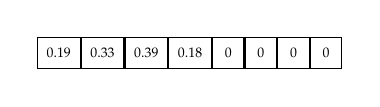
\begin{tikzpicture} [
                    cell/.style={draw, minimum width={4mm}, minimum height={4mm}, solid, thin}
                ]
                \matrix [nodes=draw]
                {
                \node [cell] {\tiny 0.19}; & \node [cell] {\tiny 0.33};   & \node [cell] {\tiny 0.39}; & \node [cell] {\tiny 0.18}; & \node[cell]  {\tiny 0};  & \node[cell]  {\tiny 0}; & \node [cell] {\tiny 0}; & \node [cell] {\tiny 0};\\
            };
                \end{tikzpicture} 
            };
        \end{tikzpicture} 
    };
    
    \draw[edge] (eventTemplates) -- (0, -8) node [midway, fill=white] {\footnotesize \textcolor{customGreen}{feature extraction}};
    

\end{tikzpicture}
   \caption{An example of encoding log sequence into two types of feature vectors: \textit{Event count vector} and \textit{TF-IDF vector}. We assume that there is $8$ event templates in the collection, thus the output vectors are also of length $8$.}
	\label{fig:feature-extraction}
	}
\end{figure}

\begin{table}
\centering
\resizebox{\textwidth}{!}{\begin{tabular}{@{}ccc@{}}
\toprule
\textbf{Matrix type} & \textbf{Row}               & \textbf{Column}                                          \\ \midrule
\textbf{\textcolor{customRed}{Event count}}    & log sequence & Frequency of event type in the log sequence              \\
\textbf{\textcolor{customRed}{TF-IDF}}         & log sequence & IDF weighted frequency of event type in the log sequence \\ \bottomrule
\end{tabular}}
\caption{A summary of feature matrix types using in our thesis }\label{tab:embeddings-summary}
\end{table}

\subsubsection*{Event Count Matrix}
A simple approach to obtain such representation is to create a event count vector for each log sequence. In other words, for each log sequence, we count the number of event type identifiers and store it as a row vector of an event count matrix. The length of the vector corresponds with the number of unique event types detected in the log parsing section, and each component of the vector corresponds to one event type. The value at each position in the vector is the frequency of event types. For event types that did not occur in the log sequence, the value is zero. Thus, one row of the event count matrix represents a single log sequence. The valuable information contributing to the machine learning model behind the event count matrix is determining what is a normal count of events and what does it mean to deviate from the normal counts.

%http://essay.utwente.nl/83142/1/Ma_MA_FacultyOfEEMathematicsAndCS.pdf illustration

This way of constructing the event count matrix is known in the literature as a natural language processing (NLP) model for feature extraction called \textit{Bag-of-Words} (BoW) \cite{informationRetrieval2008}. BoW treats each log sequence as a \textit{document} and for each \textit{word} (in our case, a word is an event type) in a document, a \textit{weight} is assigned. The weight depends on the number of occurrences of the term in the document. The length of the vector corresponds with the number of unique words in the database (analogous to all parsed event types). Then the weight score is referred to as \textit{Term Frequency} (TF) and denoted as $tf_{t,d}$, where the subscript $t$ refers to term (event type) and $d$ refers to document (log sequence) and $f_{t,d}$ is a frequency of term $t$ in document $d$. Term frequency describes the importance of an event type in a log sequence.

\begin{gather}
    tf_{t,d} = \dfrac{f_{t,d}}{\sum_{t'}f_{t', d}}
\end{gather}

In other words, $tf_{t, d}$ is the probability of occurrence of $t$ in $d$.

\subsubsection*{TF-IDF}
Another weighting scheme widely used in Information Retrieval is called \textit{term frequency–inverse document frequency} (TF-IDF). 

Using only the standard term frequency, we have to deal with an important issue. From the definition of term frequency, all event types are considered equally important \cite{informationRetrieval2008}. However, we would also like to know how important a term is not only in one document, but in the whole dataset. That's where another weight score, \textit{inverse document frequency} (IDF) comes to play. First, let us define \textit{document frequency} (DF). Document frequency $df_t$ is defined as the number of documents in the collection that contain the term $t$. Then the inverse document frequency $df_t$ of the term $t$ is defined as: 

\begin{gather}
    idf_t = \log{\dfrac{N}{df_t}}
    \label{formula:idf}
\end{gather}

where $N$ is the total number of documents in the collection. We can observe that if a term is rarely occurring in the collection, the $idf$ is high, and if the term is frequent, then the $idf$ is low.

By the definition, TF-IDF weighting of a term $t$ in document $d$ is a product of two quantities: the term frequency $tf_t$ and the inverse document frequency $idf_t$:

\begin{gather}
    tf\text{-}idf_{t, d} = tf_{t,d} \times idf_t
    \label{formula:tfidf}
\end{gather}

The intuition behind the components of TF-IDF weight is that the term frequency gives higher weight to terms that are frequently occurring in a single document. On the contrary, inverse document frequency gives lower score to words that are frequently occurring in the whole collection, as we are more interested in those that happen rarely. Thus, the $tf\text{-}idf_{t, d}$ weight of the term $t$ in document $d$ is 

\begin{enumerate}
    \item higher, if the term $t$ is frequently occurring in the small number of documents
    \item lower, if the term $t$ is rarely occurring in the high number of documents or if the term $t$ is rarely occurring in the document $d$
    \item lowest, if the term $t$ occurs in all of the document in the collection
\end{enumerate}

As a result, the feature vector of the log sequence is a vector with the value of each dimension defined by \ref{formula:tfidf}.

Final log sequence vectorization contains normalization of IDF weight by scaling between 0 and 1. There are several ways to normalize IDF, but we decided to use a common approach of applying \textit{logistic} (sigmoid) function to normalize IDF:

\begin{align*}
    tf\text{-}idf_{t, d} &= tf_{t,d} \times \sigma(idf_t) \\
    \sigma(x) &= \dfrac{1}{1 + e^{-x}}
\end{align*}

\subsubsection*{TF-IDF example}
We will show an example of how TF-IDF is computed in our case, where we work with log sequences instead of documents and event type identifiers instead of terms. Let's assume we have a collection of log sequences and we extracted $8$ event templates from our dataset. Each log message found in log sequence is marked by its corresponding event type identifier starting from $1$ to $8$, as shown in Table \ref{tab:tfidfexample1}.

\begin{table}
\centering
\begin{tabular}{@{}C{10cm}C{10cm}@{}}
\toprule
\textbf{Log sequence ID} & \textbf{Event Types} \\ \midrule
$l_1$                       & {$[1, 4, 1, 3, 7]$}               \\
$l_2$                         & {$[3, 3, 3, 8, 4]$}               \\
$l_3$                         & {$[2, 7]$}               \\
$l_4$                         & {$[3, 3, 6, 8, 4, 6]$}               \\ \bottomrule
\end{tabular}
\caption{An example of log sequences, which comprises different amounts of log messages. Log message is represented by the event type identifier.}\label{tab:tfidfexample1}
\end{table}

In order to compute the term frequency, we find the frequencies of event types in each log sequence and then normalize the frequencies to get the row vectors sum up to $1$. To continue with our example set of log sequences, the TF score computation is described in Table \ref{tab:tfidfexample2}.

\begin{table}[!h] 
\begin{subtable}[b]{1\textwidth}
\centering
  \begin{tabular}{@{}ccccccccc@{}}
        \toprule
        \backslashbox{Log sequence ID}{Event type ID} & \textbf{1} & \textbf{2} & \textbf{3} & \textbf{4} & \textbf{5} & \textbf{6} & \textbf{7} & \textbf{8} \\ \midrule
        $l_1$                     & 2          & 0          & 1          & 1          & 0          & 0          & 1          & 0          \\ \midrule
        $l_2$                     & 0          & 0          & 3          & 1          & 0          & 0          & 0          & 1          \\ \midrule
        $l_3$                     & 0          & 1          & 0          & 0          & 0          & 0          & 1          & 0          \\ \midrule
        $l_4$                     & 0          & 0          & 2          & 1          & 0          & 2          & 0          & 1          \\ \bottomrule
        \end{tabular}
        
        \caption{Computation of the frequency $f_{t,d}$ of term $t$ in document $d$.}
    \end{subtable} \\
	\hfill
	\\
    \begin{subtable}[b]{1\textwidth}
    \centering
      \resizebox{\textwidth}{!}{\begin{tabular}{@{}ccccccccc@{}}
        \toprule
        \backslashbox{Log sequence ID}{Event type ID} & \textbf{1} & \textbf{2} & \textbf{3} & \textbf{4} & \textbf{5} & \textbf{6} & \textbf{7} & \textbf{8} \\ \midrule
        $l_1$                     & 2/5          & 0          & 1/5          & 1/5          & 0          & 0          & 1/5          & 0          \\ \midrule
        $l_2$                     & 0          & 0          & 3/5          & 1/5          & 0          & 0          & 0          & 1/5          \\ \midrule
        $l_3$                    & 0          & 1/2          & 0          & 0          & 0          & 0          & 1/2          & 0          \\ \midrule
        $l_4$                     & 0          & 0          & 1/3          & 1/6          & 0          & 1/3          & 0          & 1/6          \\ \bottomrule
        \end{tabular}}
        \caption{Computation of the TF score $tf_{t,d} = \dfrac{f_{t,d}}{\sum_{t'}f_{t', d}}$.}
    \end{subtable}%
    \caption{Computation of the TF score.}
	\label{tab:tfidfexample2}
\end{table}

To compute the IDF, we first calculate the document frequency $df_t$ of each term and use the formula \ref{formula:idf} to obtain the inverse document frequencies. We will leave out the normalization for illustration purposes.

\begin{table}[!h] 
\begin{subtable}[b]{1\textwidth}
\centering
  \begin{tabular}{@{}ccccccccc@{}}
        \toprule
        \backslashbox{Log sequence ID}{Event type ID} & \textbf{1} & \textbf{2} & \textbf{3} & \textbf{4} & \textbf{5} & \textbf{6} & \textbf{7} & \textbf{8} \\ \midrule
        \textbf{$l_1$}                     & 2          & 0          & 1          & 1          & 0          & 0          & 1          & 0          \\ \midrule
        \textbf{$l_2$}                     & 0          & 0          & 3          & 1          & 0          & 0          & 0          & 1          \\ \midrule
        \textbf{$l_3$}                     & 0          & 1          & 0          & 0          & 0          & 0          & 1          & 0          \\ \midrule
        \textbf{$l_4$}                     & 0          & 0          & 2          & 1          & 0          & 2          & 0          & 1 \\ \midrule
        $\mathbf{n_t}$                  & 1          & 1          & 3          & 3          & 0          & 1          & 2          & 2         
        \\ \bottomrule
        \end{tabular}
        
        \caption{Computation of the document frequency $df_{t}$ of term $t$.}
    \end{subtable} \\
	\hfill
	\\
    \begin{subtable}[b]{1\textwidth}
    \centering
      \resizebox{\textwidth}{!}{\begin{tabular}{@{}ccccccccc@{}}
        \toprule
        \backslashbox{Log sequence ID}{Event type ID} & \textbf{1} & \textbf{2} & \textbf{3} & \textbf{4} & \textbf{5} & \textbf{6} & \textbf{7} & \textbf{8} \\ \midrule
        \textbf{$l_1$}                     & 0.602          & 0,602          & 0.125          & 0.125          & 0          & 0.602          & 0.301          & 0.301         \\ \bottomrule
        \end{tabular}}
        \caption{Computation of the IDF score $idf_t = \log{\dfrac{N}{df_t}}$. In our example, $N=4$ as there are $4$ log sequences in the collection. For instance, IDF weight of the event type $1$ is calculated as $idf_1 = \log{\dfrac{4}{1}} = 0,602$.}
    \end{subtable}%
    \caption{Computation of the IDF score.}
	\label{tab:tfidfexample3}
\end{table}

The final step is calculating the product $TF \times IDF$ and the values are shown in Table \ref{tab:tfidfexample4}.

\begin{table}[!h]
    \centering
    \resizebox{\textwidth}{!}{\begin{tabular}{@{}ccccccccc@{}}
        \toprule
        \backslashbox{Log sequence ID}{Event type ID} & \textbf{1} & \textbf{2} & \textbf{3} & \textbf{4} & \textbf{5} & \textbf{6} & \textbf{7} & \textbf{8} \\ \midrule
        \textbf{$l_1$}                     & 0.2408          & 0          & 0.025          & 0.025          & 0          & 0          & 0.0602          & 0          \\ \midrule
        \textbf{$l_2$}                     & 0          & 0          & 0.075          & 0.025          & 0          & 0          & 0          & 0.0602          \\ \midrule
        \textbf{$l_3$}                     & 0          & 0.301          & 0          & 0          & 0          & 0          & 0.1501          & 0          \\ \midrule
        \textbf{$l_4$}                     & 0          & 0          & 0.042          & 0.021          & 0          & 0.201          & 0          & 0.05
        \\ \bottomrule
        \end{tabular}}
    \caption{TF and IDF scores from the example are multiplied to obtain TF-IDF}.
    \label{tab:tfidfexample4}
\end{table}

We assume that by using TF-IDF weighting, we will provide an extra information about the event type distribution not only in terms of log sequences, but also in the whole data set, that could potentially increase ML model's performance. 

\section{Anomaly Detection}

Now that we have created the feature matrices, machine learning methods can be applied to detect outliers in the data. For our experiments, we are using an open-source machine learning toolkit \textit{Loglizer}. 

\subsection{Loglizer}
\label{subscetion:loglizer}

Loglizer\footnote{https://github.com/logpai/loglizer} is an open-source machine learning based log analysis toolkit for automated anomaly detection written in Python \cite{he2016}. Loglizer was developed for automated anomaly detection as a part of LogPAI \footnote{\url{http://www.logpai.com}}, which is a collection of AI-based log analytics solutions. These log analysis tools have been used by industrial teams in Microsoft and Huawei. It includes three supervised anomaly detection models (\textit{Logistic Regression, Decision Tree, Support Vector Machine}) and six unsupervised anomaly detection models (\textit{Local Outlier Factor, One-Class SVM, Isolation Forest, Principal Component Analysis, Invariants Mining, Clustering}). At the time of writing this thesis, another two unsupervised models were in the development (\textit{DeepLog, AutoEncoder}). 

We decided to leverage a third-party toolkit for several reason. Firstly, as the algorithms we are using in our experiments have been already implemented, there is no need to completely reinvent the wheel and write the implementation ourselves. This way we can avoid a time consuming process and rather focus on the main intention of our research - to investigate if applying various anomaly detection techniques on a real-world dataset can lead to successful results and how to approach it.

Another benefit is that the Loglizer anomaly detectors are working with log sequences. This means that each of the models is trained on a set of log sequences, and the output of the detector classifies whether a single log sequence is an anomaly or not. As described in Section \ref{section:featureEngineering}, we use windowing for generating the log sequences, which makes the Loglizer toolkit a great fit in our research context. Specifically, four methods were used in our research: Invariants Mining, Isolation Forest and PCA. The underlying algorithms behind these tools are presented in Section \ref{section:anomalyDetectionLiteratureReview}.

Implemented anomaly detection methods are evaluated on a public dataset, HDFS. Logs in HDFS dataset were collected from Amazon EC2 platform and contain $11\,175\,629$ entries \cite{xu2009}. Loglizer provides benchmarking results on both supervised and unsupervised methods separately using this dataset, which can be found in Table \ref{table:loglizer}. Evaluation metrics are explained in Section \ref{section:evaluationMetrics}. Benchmarking gives a better idea of the expected performance of the anomaly detection methods we are planning to use in our work. 

Last but not least, Loglizer makes it easier to reproduce, understand and customize the experiments, as the code is open-source.

\begin{table}[h]
\centering
\begin{tabular}{@{}cccc@{}}
\toprule
\multicolumn{4}{c}{\textbf{HDFS}} \\ 
\textbf{Model}    & \textbf{Precision} & \textbf{Recall} & \textbf{F1} \\  \toprule \midrule
\multicolumn{4}{c}{\textit{Supervised Methods}}                        \\ \midrule
LR                & 0.955              & 0.911           & 0.933       \\
Decision Tree     & 0.998              & 0.998           & 0.998       \\
SVM               & 0.959              & 0.970           & 0.965       \\ \midrule
\multicolumn{4}{c}{\textit{Unsupervised Methods}}                      \\ \midrule
LOF      & 0.967              & 0.561           & 0.710       \\
One-Class SVM     & 0.995              & 0.222           & 0.363       \\
Isolation Forest  & 0.830              & 0.776           & 0.802       \\
PCA               & 0.975              & 0.635           & 0.769       \\
Invariants Mining & 0.888              & 0.945           & 0.915       \\
Clustering        & 1.000              & 0.720           & 0.837       \\ \bottomrule
\end{tabular}
\caption{Benchmarking results of three supervised and six unsupervised anomaly detection methods on HDFS dataset \cite{he2016}}.
\label{table:loglizer}
\end{table}

\subsection{Experiment Workflow}
Running machine learning experiments is usually an iterative process, where each iteration requires different configuration parameters, input training and testing datasets and a lot of file handling. The same holds for our anomaly detection experiments. We obtained several raw datasets from the SmartConnect's system. We picked four anomaly detection methods, where each method might require a different dataset as well as its own parameter configuration. Every raw dataset needs to parsed from its initial JSON file into a unified structure, it needs to be cleaned and faulty log entries need to be removed. Then a log parser program is applied to obtain an event type identifier for each log message. Finally, we use two different feature matrix representations as an input for anomaly detection methods. After having obtained trained models for every dataset, the evaluation follows. Having so many dependent processes to perform for each experiment iteration where things can get messy very easily, makes it desirable to have an automated workflow system. Despite our thesis not being a software engineering thesis, thus the focus was not on having a perfectly extensible workflow, we attempted to come up with a solution that saves time required to run experiments.

We created a Makefile-based pipeline comprising a set of Python scripts to facilitate experiments. The goal was to have a reproducible, modular and scalable solution to deal with the complexity of conducting experiments. In this section, we will briefly describe the architecture of this pipeline and the implementation of the experiment scripts.
 
 \subsubsection*{Makefile}
The experiment execution is orchestrated by the GNU \textit{make} instructions described in the Makefile scripts. A Makefile consists of a set of rules that generate target files if any of their dependencies change. We decided to use Makefile because it directly enforces a modular character to our workflow. Every rule must follow the shape:

\begin{verbatim}
    target ... : prerequisities ... 
        recipe
        ...
\end{verbatim}

 Usually, targets and prerequisities are file names and recipes are commands. Makefile can be expressed by a directed acyclic dependency graph \cite{feldman1979make}. The dependency graph of our Makefile is illustrated in Figure \ref{fig:makefile}. 
 
 Each target contained in the Makefile operates on the \texttt{DATASET} variable assignment. \texttt{DATASET} represents the name of the dataset, that needs to exist in the \texttt{data/raw/} directory of the project folder before any of the targets are run, therefore we call it a \textit{prerequisity} or a \textit{dependency}. The variable can be set from outside of the Makefile as part of the command line. Changing the value of \texttt{DATASET} directly influences the names of the generated output files. By running \texttt{make} in the directory containing Makefile and assigning \texttt{DATASET} variable, we can manage the experiment workflow:
 
 \begin{itemize}
     \item \texttt{make} \textit{data} \texttt{DATASET=<dataset name>}
     \begin{itemize}
         \item Parses JSON file with raw data into a panda's DataFrame
         \item Flattens columns of the DataFrame that contain nested JSON structures
         \item Executes log abstraction by processing log messages, extracting an event type for each log message and appending event type column to the DataFrame
         \item Stores DataFrame with preprocessed logs 
         \item Extracts event count and TF-IDF feature matrices
         \item Stores feature matrices
     \end{itemize}
     \item \texttt{make} \textit{train} \texttt{DATASET=<dataset name>}
     \begin{itemize}
         \item Executes training script and generates invariant mining, isolation forest, log clustering and PCA models using event count and TF-IDF feature matrices
         \item Stores models
     \end{itemize}
     \item \texttt{make} \textit{evaluate} \texttt{DATASET=<dataset name>}
     \begin{itemize}
         \item Executes evaluation script for invariant mining, isolation forest, log clustering and PCA models trained using event count and TF-IDF feature matrices by detecting anomalies on provided labeled dataset
         \item Generates precision, recall and F1 score into CSV files stored in \texttt{\justify results/metrics} directory
         \item Generates labels predicted by all the models into CSV files stored in~\texttt{results/predictions} directory
     \end{itemize}
     \item \texttt{make} \textit{all} 
     \begin{itemize}
         \item Runs all modules of the workflow
     \end{itemize}
     \item \texttt{make} \textit{clean} \texttt{DATASET=<dataset name>}
     \begin{itemize}
         \item Cleans up all generated files related to \texttt{DATASET} including the trained model, if it exists
     \end{itemize}
 \end{itemize}
 
 \begin{figure}[!h] \centering {
   \begin{tikzpicture} [
    edge/.style={-latex,shorten >=1pt, thin, color=customGrey},
    line/.style={-,shorten >=1pt, thin, color=customGrey},
    fileTarget/.style={rectangle, draw=customBlue, align=left, minimum width=55mm, minimum height=7mm},
    phonyTarget/.style={rectangle, draw=customRed, align=left, minimum width=20mm, minimum height=7mm}
]

\node[fileTarget, align=center] (root) at (0, 0) {\tiny data/raw/\$(DATASET).json};

\node[fileTarget, align=center] (preprocessed_tf) at (-3, -1.5) {\tiny data/preprocessed/tf/\%-preprocessed.pickle};

\node[fileTarget, align=center] (preprocessed_tfidf) at (3, -1.5) {\tiny data/preprocessed/tfidf/\%-preprocessed.pickle};

\draw[edge] (root) -- (preprocessed_tf);
\draw[edge] (root) -- (preprocessed_tfidf);

\node[fileTarget, align=center] (features_tf) at (-3, -3) {\tiny data/features/tf/\%.npy};

\node[fileTarget, align=center] (features_tfidf) at (3, -3) {\tiny data/features/tfidf/\%.npy};

\draw[edge] (preprocessed_tf) -- (features_tf);
\draw[edge] (preprocessed_tfidf) -- (features_tfidf);

\node[phonyTarget, align=center] (data) at (0, -4.5) {\tiny data};

\draw[edge] (features_tf) -- (data);
\draw[edge] (features_tfidf) -- (data);

\node[fileTarget, align=center] (model_tf) at (-3, -6) {\tiny models/tf/\%.model};

\node[fileTarget, align=center] (model_tfidf) at (3, -6) {\tiny models/tfidf/\%.model};

\draw[edge] (features_tf) -- (model_tf);
\draw[edge] (features_tfidf) -- (model_tfidf);

\node[phonyTarget, align=center] (train) at (0, -7.5) {\tiny train};

\draw[edge] (model_tf) -- (train);
\draw[edge] (model_tfidf) -- (train);

\node[fileTarget, align=center] (results) at (0, -9) {\tiny results/\%.csv};

\draw[edge] (model_tf) -- (results);
\draw[edge] (model_tfidf) -- (results);

\node[phonyTarget, align=center] (evaluate) at (0, -10.5) {\tiny evaluate};

\draw[edge] (results) -- (evaluate);

\node[phonyTarget, align=center] (all) at (0, -12) {\tiny all};

\draw[edge] (evaluate) -- (all);

\end{tikzpicture}
   \caption{A dependency graph for a Makefile to run experiments in our thesis. Blue rectangles represent the \textit{file targets} and the red rectangles represent \textit{phony targets}. Phony targets are are targets that are not creating or updating a file, but they represent a name for a sequence of commands to be executed. Phony targets allow our experiments to be executed in a modular manner.}
	\label{fig:makefile}
	}
\end{figure}

Models and their configurations, that will be trained in the pipeline, can e specified from inside of the Makefile.

\subsubsection*{Scripts Implementation}
 Having a consistent file naming convention and a consistent file organization into directories and subdirectories is crucial for automated experiments. The example of our experiment directory structure that is designed for use with Makefile is in the Appendix \ref{appendix:dir_structure}.
 
 Each machine learning method has three Python scripts in the \texttt{src/models} directory: \textit{train}, \textit{evaluate} and the \textit{model} itself. 
 
 Each \textit{model} script functions as a wrapper with a common interface, that contains algorithm providing library (in our case, we are using LogLizer library, as described in Section \ref{subscetion:loglizer}) and enables calling the following methods:
 
\begin{itemize}
    \item \texttt{\_\_init\_\_}
    \item \texttt{fit}
    \item \texttt{predict}
    \item \texttt{evaluate}
    \item \texttt{save}
    \item \texttt{load}
\end{itemize}

The advantage of having a wrapper above the actual model is that it can be easily replaced by other library providing the model implementation, or we can provide our own implementation.

As one can see from the list above, each model also contains \texttt{save} and \texttt{load} methods. They are included in the model as a mean of serialization and deserialization of the trained model. The reason for that is the fact that training a model is usually a very time consuming task. Being able to load an already trained model saves us the trouble of training the model every time it is required. A serialized model can be conveniently restored later and used for evaluation or prediction. We use \texttt{pickle}\footnote{https://docs.python.org/3/library/pickle.html} library, that converts arbitrary Python's object into a byte stream. The process of serializing the data is then referred to as "pickling" and deserializing as "unpickling".

\textit{Train} scripts allow optional and model-specific parameters to tune the models. These parameters can be modified in the Makefile. Then they simply load the preprocessed data, instantiate the model and execute the model training process. Finally, the trained model is stored into a pickle. 
 
\textit{Evaluate} scripts contain loading the trained model and running the \texttt{\justify evaluate} method to obtain metrics and predictions.

As shown in the directory structure in the Appendix \ref{appendix:dir_structure}, preprocessed features, trained models and resulting metrics and predictions are stored in either \texttt{tf} or \texttt{tfidf} folder, depending to which feature extraction method the particular file belongs. \texttt{tf}, as an abbreviation for term frequency, is an equivalent of what we call in our thesis an \texttt{event count}, as we explained in detail in Section \ref{subsection:features}. We use \texttt{tf} in our file structure for the benefit of brevity.

\subsection{Mapping from Prediction Back to Log Entry}
Once the output is computed, what we obtain is a prediction for each window of the input dataset. This is true regardless of the specific machine learning model used for the computation. 
This kind of output that consists from ones and zeros is not very helpful if we want to understand why we got those results and if they are correct. Ideally, we want more elaborate information about the individual windows.
Typically, the interesting part would be those windows, that were identified as anomalous as they are assumed to be less frequent and more important. However, there are use cases where we want to investigate all of them, especially in the debugging phase. 

From a feature vector of a given window, only event type's ID and frequency is stated, the template and order is lost.
After discussing with domain experts what would be a valuable information about a time window, we concluded that with every window it should be also provided:
\begin{itemize}
    \item \textit{How frequent is each of the event types and what is the template of each event.}\\
    We create a histogram, ordered descending from the most frequent events to the least frequent. This gives a good overview of what is the state of the system in a given time window. 
    \item \textit{Raw trace of logs within the window.}\\
    Histogram is a good start but for some cases, details and preserved order matter. In some cases also the variable parts of log messages that are missing in the log templates need to be known to gain a clear picture of what was going on in the system. Therefore, we also assign trace of raw logs ordered by the time as they happened.
    \item \textit{What time range a window corresponds to.}\\
    It is simple to map from a window index to human readable time. This way, an expert can tell whether something special was happening in the system. For example, regular testing may take place at specific times everyday, which can explain some behaviour.
\end{itemize}
 
% Flowchart: https://bost.ocks.org/mike/make/


\chapter{Experiments}
\label{chapter:experiments}

In this chapter, we will look at the the configuration of experiments that has a direct impact on the results of our $4$ different anomaly detection approaches. Before conducting the experiments, we will also look at our data visually to check the correctness of assumptions we hold about the data. After that, we summarize the experiment setup including datasets, software and hardware used for experiments. \todo{Evaluation matrics} Finally, we present the definitions of tunable hyperparameters and provide an overview of the hyperparameter values that performed best and are used for final experiments.

\section{Exploration of Assumptions}
\todo{do we want to keep single assumptions numbered as subsections?}
To get a better insight into the dataset, it is useful to perform an initial Exploratory Data Analysis (EDA) \cite{eda} of our dataset. Exploratory data analysis is being used to analyze the underlying structure of the data and summarize the main characteristics, often via visualization methods. The visualization helps us to check our assumptions and formulate hypotheses of the data, which are important to choose the correct anomaly detection approaches. In addition, being able visualize the logs will help us answer \textbf{RQ1} (Research Question 1).

We use the numerical representation of our dataset that we obtained by feature extraction. The embedding of log sequences contains \featureVectorLength\ variables. Data of such high dimensions are difficult to interpret. Therefore, it is necessary to use Dimensionality reduction techniques. To perform an initial exploration as well as to visualize the results of anomaly detection, we will employ two algorithms, PCA and t-SNE, to reduce the dimensionality for data visualization:

\begin{itemize}
    \item \textbf{Principal Component Analysis (PCA)} \\
    One way of reducing the dimensionality of data without losing too much information is to use Principal Component Analysis (PCA) as an unsupervised tool for exploratory data analysis. 
    In PCA, the data points (in our case, feature vectors) in our\\ \featureVectorLength-dimensional feature space are transformed onto a 2-dimensional feature subspace. Furthermore, the variables in the new artificial subspace (principal components) are not correlated. The first principal component (PC1) spreads in the direction of the x-axis and explains the most variance in the data.
    
    \item \textbf{t-distributed Stochastic Neighbor Embedding (t-SNE)}\\
    t-SNE is a more recent algorithm for dimensionality reduction into a space of two or three dimensions, that is particularly well-suited for data visualization \cite{tsne}. PCA is a linear technique that keeps the dissimilar datapoints in the low-dimensional projection far apart. In contrast with PCA, t-SNE is a non-linear technique. It focuses on retaining the local structure by keeping the high dimensional datapoints that lie on or near a non-linear manifold in lower dimensions close together. Retaining local structure, while also revealing an important global structure is the biggest advantage over linear techniques, where this is usually not possible.
    
\end{itemize}

All the visualizations in the sections below were obtained on the event count embeddings of the data.  

\subsection{Daily vs Nightly}

As we explained in the earlier sections of this chapter, we train the models on the Nightly dataset under the assumption that its data points are normal. On the other hand, we have no prior assumptions about the Daily dataset and about the distributions in it. Thus, we want to perform a simple visual comparison of the Daily and Nightly dataset. Next, we sought to determine whether the data points from the day fall within the normal region.

In Figure \ref{fig:tsne-single}, there are two visualizations of applying t-SNE to the the Nightly and Daily datasets correspondingly. t-SNE analysis of the Daily dataset appears to separate the data into four visual clusters. While it is difficult to interpret what each of the clusters represents, we suppose that at the day of obtaining the Daily dataset, the developers were testing out $4$ different features \todo{restructure}, that led to the groupings of data points into clusters.

The visualization of the t-SNE in the plot of the Nightly dataset shows that most of the data points are packed together and form a cluster. However, there is a cluster of points at the bottom of the plot, that appears to be fairly distant from the rest of the points and might be considered to be a set of outliers. Upon closer inspection of the raw logs behind the data in this cluster, we discovered that they contain a high number (around $400$ hundred logs every two minutes) of log messages informing a call was happening, as illustrated by the following event templates:

\begin{itemize}
    \item \texttt{\justify Call \{1586,1\} \{:call\_number, <*> <*> forwarding audio RtpPacket\{ssrc: <*> urid: <*> timestamp: <*> seq\_num: <*>}
    \item \texttt{\justify Call \{1586,1\} \{:call\_number, <*> <*> received RtpPacket\{ssrc: <*> urid: <*> timestamp: <*> seq\_num: <*> from \{228, 28, <*> <*>}
    \item \texttt{\justify Call \{1586,1\} \{:call\_number, <*> <*> forward RtpPacket\{ssrc: <*> urid: <*> timestamp: <*> seq\_num: <*> LMR: [ssrc: <*> urid: <*> to \{228, 28, <*> <*>}
\end{itemize}

This is further confirmed by visualizing the Call dataset in respect to the Nightly dataset.

As calls are not happening frequently during the testing phase, comparing to other processes that are happening in the system, this is precisely what we expect to be reflected in the logs. Nevertheless, as shown in the plot, the cluster is considerably distant from the rest of the points and we do not want regular calls to be detected as anomalies. Here it is important to note that the distances between clusters in t-SNE do not 
necessarily have to mean something. To obtain clusters that retain global geometry, it is required to fine-tune the \textit{perplexity} hyperparameter of t-SNE. Thus, we do not know where does the assumed call cluster lies with respect to the rest of the data points.


% highest along the y-axis, which is the second principal component, and it represents only roughly $19\%$ of the information. 


\begin{figure}%
    \centering
    \subfloat[\centering Nightly Dataset]{{\includegraphics[width=5.52cm]{img/tsne-nightly.pdf} }}%
    \qquad
    \subfloat[\centering Daily Dataset]{{\includegraphics[width=5.52cm]{img/tsne-daily.pdf} }}%
    \caption{Application of t-SNE on the event count vector embeddings of the Nightly and Daily datasets.}%
    \label{fig:tsne-single}%
\end{figure}

Finally, we are interested to see how does the PCA performs in comparison to t-SNE and we also want to plot both Daily and Nightly dataset with respect to each other. Figure \ref{fig:pca-nightly-daily} displays a plot of the first two principal components after performing principal component analysis on the Nightly and Daily dataset. Figure \ref{fig:tsne-nightly-daily} is a t-SNE plot visualizing the Nightly and Daily datasets.

The points produced by PCA appear to be much more crowded in comparison with t-SNE, however in both plots there is a very little intersection between Daily and Nightly data. One way to explain this is that the tests performed during the night do not completely cover the behaviour of the system. Another explanation, that was confirmed by the developers at Motorola as the most likely, is that the experiments performed during the day vary each day depending on the feature that is being tested and it may also behave completely counter to what we consider a normal behaviour. Nevertheless, these visualizations confirmed, that the Daily dataset should not be used for training the models as it's unpredictable and inconsistent. It is still a good candidate for performing dual validation, where an expert's understanding of underlying processes will help us understand the anomaly detection models. \todo{elaborate}.

\begin{figure}[h]
    \centering
    \includegraphics[width=\textwidth]{img/pca-nightly-daily.pdf}
    \caption{Application of PCA to the Daily and Nightly dataset}
    \label{fig:pca-nightly-daily}
\end{figure}

\begin{figure}[h]
    \centering
    \includegraphics[width=\textwidth]{img/tsne-nightly-daily.pdf}
    \caption{Application of t-SNE to the Daily and Nightly dataset}
    \label{fig:tsne-nightly-daily}
\end{figure}

\subsection{Completeness of the Nightly dataset}
\todo{is completeness the right word}
Another set of important questions we would like to answer by conducting EDA are concerning the completeness of Nightly dataset obtained on 24 January, 2021, that we plan to use for one-class model training: \textit{Do data from nightly testing differ among different dates?} \textit{Would merging data from several nightly testing datasets provide some extra information about the normal behaviour of the system?}

To analyze the data and answer these questions, we will again use PCA and t-SNE and plot data obtained during two different nights of testing. Figure \ref{fig:tsne-nights-comparison} gives the visualization of the results. We can observe that the two datasets overlap almost entirely in both PCA and t-SNE plots. From the substantial overlap we can safely assume that logs gathered during the nightly testing are equivalent within the different dates.

By our domain knowledge, we know that the code under the tests is going to slightly differ, as the software product of Motorola SmartConnect is being developed. The reason is that master branches of services are being tested and we do not expect them to be changing dramatically day to day. 
However, it is something that has to be taken into account when deploying our solution. It has to be verified that the code whose produced logs are being analyzed by our anomaly detection algorithm is also the version of code that runs the tests.

We conclude that using data from just one night is enough for training the anomaly detection models and adding more logs from different nights would not bring any extra information to the data. 

\begin{figure}%
    \centering
    \subfloat[\centering PCA]{{\includegraphics[width=5.52cm]{img/pca-nights-comparison.pdf} }}%
    \qquad
    \subfloat[\centering t-SNE]{{\includegraphics[width=5.52cm]{img/tsne-nights-comparison.pdf} }}%
    \caption{Comparing data from nightly testing obtained from two different dates.}%
    \label{fig:tsne-nights-comparison}%
\end{figure}


\subsection{Call Cluster}
In the t-SNE of the Nightly dataset, we could see a cluster of points that we assumed are calls being made between two radios. The assumptions stems from us choosing several random data points (log sequences) from that cluster and hand-checking the histogram of log templates within the log sequences for those representing calls. We want to prove that it is a cluster of call logs and it is not an unknown anomaly. We will prove this assumption by highlighting the Glostrup Calling dataset created specifically for this purpose in the t-SNE embedding of the Nightly dataset as a central point of reference about where do the call data points cluster.

Figure \ref{fig:tsne-nightly-calls} is depicting running t-SNE on the above described scenario. After applying feature extraction into $2$ minute windows on the simulated $8$ minutes of calls, we obtain $4$ data points (highlighted by green color). The visualization of the plot indicates that the call data points fall very close to the observed cluster and in addition, all of the call data points are consistently tightly packed together. 

Therefore, we believe that it is possible to determine the class of a clustered group of data points even without leveraging the actual labels. It confirms our assumption that the data from the Nightly dataset are anomaly free and that the observed cluster is indeed a cluster of calls.

\begin{figure}[h]
    \centering
    \includegraphics[width=\textwidth]{img/tsne-nights-call-comparison.pdf}
    \caption{Application of t-SNE to the Nightly and Glostrup Calling dataset.}
    \label{fig:tsne-nightly-calls}
\end{figure}

\subsection{Anomalies}
The last assumption which we want to verify before using the data to train actual machine learning models and considerably the most important one, is to look whether anomalies have a tendency to cluster together in different regions than normal data. It is crucial, because if human eye can detect an anomaly by looking at a plot, then we can assume that anomaly detection algorithms should be also able to detect these anomalies. 

In order to prove that, we will plot our Anomalies dataset generated by collecting anomalies during simulation of anomaly scenarios described in Section \ref{anomaly_types}. In both PCA and t-SNE plots in Figure \ref{fig:pca-anomalies} and \ref{fig:tsne-anomalies} respectively, anomaly of killing the Redis is represented by green and killing the RabbitMQ is represented by blue color. Anomalous data points are plotted in respect to normal points, which are highlighted as red. 

Both plots give us a clear picture that the data points are split into distinct clouds of the same anomaly types. Moreover, the anomalous points are located outside of the normal region. We consider the fact that different anomalies can be succesfully distinguished as clusters in the embedding space as an answer to the \textbf{RQ1}. In this case, it is clear that t-SNE gives us better clustering result than PCA with less point overlapping each other, even thought both techniques are able to separate the data points into different classes. However, it is interesting to see in the PCA plot, that the Killing Redis anomaly is located much closer to the cluster of normal points than Killing RabbitMQ (as mentioned earlier, we should not take the distances between clusters in t-SNE plots into account unless tuning its parameters, that's why we focus on the PCA graph for cluster proximity analysis). This can be explained as an outage of all brokers in the distributed architecture of the system that relies on passing messages between microservices causes a major distortion of the whole infrastructure. 
While non-functioning Redis cache is an issue that can be overcome relatively easily, the latter one causes severe problem in the application, propagating to many places. Also, as we observed, the broken broker scenario makes the system disfunctional for a much longer time period giving services longer window for generating greater amount of logs indicating problems.

We got a solid indication that the feature embedding is informative enough to identify anomaly clusters.

\begin{figure}[!h]
    \centering
    \includegraphics[width=\textwidth]{img/pca-anomalies-vs-normal.pdf}
    \caption{Application of PCA to the anomaly data.}
    \label{fig:pca-anomalies}
\end{figure}

\begin{figure}[!h]
    \centering
    \includegraphics[width=\textwidth]{img/tsne-anomalies-vs-normal.pdf}
    \caption{Application of t-SNE to the anomaly data.}
    \label{fig:tsne-anomalies}
\end{figure}

\section{Evaluation metrics}
\label{section:evaluationMetrics}
In order to appropriately compare different anomaly detection algorithms and different experiment settings, evaluation metrics are required.

Firstly, let's introduce four basic metrics: true positive (TP), false positive (FP), true negative (TN) and false negative (FN). 

To give an example, let's consider an experimental setting: in a classification task, for each data example we have assigned a binary label $l$ with values in a set of classes. It is important to note that one class, that is usually positive, is of special interest, for which the evaluation measure is valid. It gives an information about the correctness of the example given the anomaly detection task. Moreover, an anomaly detector produces a prediction $\hat{l}$, assigning for each data example whether it classifies it as an anomaly or a normal data instance. The pair-wise relationship the four counts is explained by the confusion matrix in Table \ref{table:confusionMatrix}. Confusion matrix is a form of contingency table, that allows interpretation of classifier's performance on a labeled dataset. It is a $2 \times 2$ matrix (in case of having only two classes, but can be easily extended for multiple classes), where rows represents an actual value of a variable, while columns represent the predicted value of a variable.

\begin{table}[!h]
\centering
\begin{tabular}{cccc}
\multicolumn{1}{r}{}                 &                              & \textbf{Predicted}          &   $\hat{l}$                          \\ \cline{3-4} 
                                     & \multicolumn{1}{l|}{}        & \multicolumn{1}{l|}{Anomaly} & \multicolumn{1}{l|}{Normal} \\ \cline{2-4} 
                                      
\multicolumn{1}{l|}{\textbf{Actual}} & \multicolumn{1}{l|}{Anomaly}  & \multicolumn{1}{l|}{\textcolor{customBlue}{\textbf{TP}}}     & \multicolumn{1}{l|}{\textcolor{customRed}{\textbf{FN}}}      \\ \cline{2-4} 
\multicolumn{1}{c|}{\textit{l}}                & \multicolumn{1}{c|}{Normal} & \multicolumn{1}{l|}{\textcolor{customDarkRed}{\textbf{FP}}}     & \multicolumn{1}{l|}{\textcolor{customGreen}{\textbf{TN}}}     \\ \cline{2-4} 
\end{tabular}
\caption{An example of a confusion matrix for binary classification.}
\label{table:confusionMatrix}
\end{table}
 
Many meaningful measures can be extracted out of the confusion matrix. The evaluation measures are calculated on the positive class, which is assumed to represent the presence of an anomaly.

\textit{Accuracy} is the most general metrics to measure performance. It simply measures the fraction of correct predictions from all the available data points. The computation of accuracy in binary classification is done as shown in the following equation:

\begin{align}
    Accuracy = \dfrac{TP + TN}{TP + TN + FP + FN}
\end{align}

However, accuracy alone does not exactly reflect the real performance of a system designed to correctly detect anomalies. It does not differentiate between the number of correct predictions of different classes \cite{performanceEvaluation2006}. The reason why accuracy measure is not enough in the majority of ML applications will be explained in the remainder of this section. 

The most typically used metrics for estimating performance in machine learning are \textit{precision, recall} and ${F_{\beta}-measure}$. They measure the correct prediction of anomaly within different classes. In our research, we will also focus on these three  performance indicators.

In order to use them, the problem for which we want to estimate performance must be a classification problem. We assume our dataset represents a normal behaviour of the system, thus an anomaly detection problem can be translated into a one-class classification problem. 

Precision, recall and $F_{\beta}$-measure rely on the ratios of TP, FP, TN and FN counts. 

Precision represents the fraction of correctly detected anomalies from the total number of reported anomalies. Recall measures the fraction of correctly detected anomalies from the total number of anomalous data points in the dataset. Lastly, $F_{\beta}$-measure combines both of these measures into a single measure. $F_{\beta}$-measure represents the harmonic mean of precision and recall. If precision and recall are evenly balanced, then $\beta = 1$ and we call it F1-measure. If $\beta > 1$, the score is in favour of precision. On the other hand, it is in favour of recall if $\beta < 1$. 

Let's look at the mathematical formulas for calculating evaluation measures:

\begin{align}
    Precision &= \dfrac{TP}{TP + FP} \\
    Recall &= \dfrac{TP}{TP + FN} \\
    F_{\beta}-measure &= (\beta^2 + 1) \cdot \dfrac{Precision \times Recall }{\beta^2 \cdot Precision + Recall} 
\end{align}

The reason for $F_{\beta}$ score is that improving either precision or recall on their own is a trivial task, but the goal is to optimize both of them at the same time. Accuracy metrics is more useful when true positives and true negatives are more important. However, false positives and false negatives are considered to be crucial in most of the classification problems. Thus, in these cases, $F_{\beta}$ score happens to be a better evaluation metrics. False negatives and false positives are given more weight while not letting large numbers of true negatives to influence the score.

In addition, as anomalies occur much less frequently than normal data samples, we can easily achieve a high accuracy without catching anomalies. That's why we will not use accuracy metrics for evaluation in this thesis.

\todo{ROC curve evaluation?}
%https://reader.elsevier.com/reader/sd/pii/S0167404818306333?token=86A40DFE4370A7717E0B15DEAAD2B345D4CC6B9710DBAF61E109BBCB91AF725627908E3B8838A3472D5D1E42201C1845

\section{Experimental Setup}
\label{section:experimental-setup}
In Chapter \ref{chapter:literatureReview}, we have described four anomaly detection algorithms: Isolation Forest (\ref{section:lrIsolationForest}), PCA (\ref{section:lrPCA}), Invariant Mining (\ref{section:lrInvariantMining}) and Log Clustering (\ref{section:lrLogClustering}). These algorithms will be used to carry out the unsupervised anomaly detection experiments. In this section, we will describe the data used in these experiments and discuss the choice of different parameters for each of the anomaly detection methods. To tune the parameters, we will use the evaluation metrics described in previous section.

\subsection{Dataset}
The dataset used for training models is the Nightly dataset with data instances of normal class, thus we also refer to this type of learning as one-class learning. Before training, in all of our experiments indistinguishably, we start by preprocessing data into numerical vector embeddings following the methods described in Chapter \ref{methodology}. In Table \ref{tab:training} we give an overview of the statistics regarding the dataset used for training and testing.

We used the sliding window technique to divide the dataset into log sequences. The number of resulting sequences depends on the size of the window and a size of the step.  The window size should be set such that it contains the maximal amount of information. We have identified that the anomalies we observe in the experiments spawn at most two minutes. Therefore, we set the window size to two minutes, and the step size into two minutes as well, so that no two windows overlap. As a result we got $201$ log sequences extracted out of the Nightly dataset. Each log sequence can be one of two different vector representations: \textit{event count} vectors and \textit{TF-IDF} weighted vectors. Thus, we will run each experiment twice on both embedding types.

The length of a vector is given by the number of unique event templates, that were extracted and stored in our log template miner's state during the preprocessing of all datasets used in our research. Thus, by the time of model training, the number of event types as well as the length of each log sequence is equal to $3\,963$.

% Please add the following required packages to your document preamble:
% \usepackage{booktabs}
% Please add the following required packages to your document preamble:
% \usepackage{booktabs}
\begin{table}[h]
\centering
\resizebox{\textwidth}{!}{\begin{tabular}{@{}ccccc@{}}
\toprule
\textbf{Dataset} & \textbf{Window size} & \textbf{\# Log sequences} & \textbf{\# Event types} & \textbf{Ratio of anomalies} \\ \midrule
Nightly          & 2 minutes            & 201                       & 3693                    & 0                           \\
Testing          & 2 minutes            & 131                       & 3693                    & 0.22                        \\ \bottomrule
\end{tabular}}
    \caption{Summary of statistics of the Nightly dataset used for training and Testing dataset used for model evaluation and hyperparameter tuning.}
    \label{tab:training}
\end{table}

\subsection{Software}
To develop data preprocessing scripts and to conduct our experiments, Python 3.6.9 was used as a primary programming language. In addition, we used the following Python libraries: 

\begin{itemize}
    \item pandas 1.1.3
    \item numpy 1.19.2
    \item torch 1.7.1
    \item plotly 4.12.0
    \item matplotlib 3.3.2
    \item jupyterlab 2.2.8
\end{itemize}

Exploratory analysis, data plotting and the preparations of scripts for the ML pipeline are performed using Jupyter Notebook with a Jupyter Lab interface for browsing files. Jupyter Notebook is a web-based interactive computational environment for writing python code, that operates in a web-based environment. The biggest advantage in using Jupyter Notebook instead of writing Python scripts directly is the ability to execute inline code and see the result directly beneath it. It also allows to add formatted texts that improves the readability and reasoning behind the analysis steps.

\subsection{Hardware}
All experiments were conducted on a HP ZBook machine with the following technical specification:
\begin{itemize}
    \item Operating System: Linux Mint 19.3 Cinnamon
    \item CPU: Intel Core i7-8850H
    \item RAM Size: 32 GB
    \item CPU Frequency: 2.60 GHz
    \item Internal Storage: 500 GB
\end{itemize}

\subsection{Algorithm Hyperparameters}
Hyperparameters are the values of parameters that are used to configure a machine learning model and they must be set before the learning process, which is the main difference between parameters, which are found \textit{during} the learning process. As the performance of the model on given combination of dataset and hyperparameters is not known, it is required to explore the range of possible values to obtain optimal hyperparameters. This optimization process is called \textit{tuning}.

The strategy we follow to find optimal parameters is a simple grid search: For each combination of hyperparameter values, we train a model and look at the evaluation metrics for comparison.

Below, we provide a list of hyperparameters and their definitions for all algorithms. The list of values for which they are tested can be seen in Table \ref{tab:hyperparameters}.


\subsubsection*{Isolation Forest}
\begin{enumerate}
    \item \textbf{Number of estimators}: The number of isolation trees that will be generated in the isolation forest, also referred to as the number of base estimators in the ensemble.
    \item \textbf{Max samples}: The number of samples that will be drawn from the input matrix for training each of the iTrees. This number cannot be higher than the number of samples in the input dataset. 
    \item \textbf{Contamination}: Percentage of points in our data sets that are anomalous. The value of contamination parameter is used during fitting, when the threshold on the decision function is being defined.
    \item \textbf{Max features}: This parameter enables us to control the number of features to be drawn from the dataset to train each of the iTrees. The maximum value is the number of features in the dataset. 
\end{enumerate}

\subsubsection*{PCA}
\begin{enumerate}
    \item \textbf{Number of components}: Number of output features (principal components) to be extracted in PCA. If a decimal number is provided, it is used to represents the variance ratio than the principal components cover
    \item \textbf{Threshold}: The threshold for anomaly detection scores, which is a value between $0$ and $1$. When this values is exceeded, the sample is considered an anomaly. The value of the threshold can be set to be calculated automatically using Q-statistics using the value of the alpha hyperparameter
    \item \textbf{Alpha}: The alpha values for Q-statistics for calculating anomaly detection threshold. 
\end{enumerate}

\subsubsection*{Invariants Mining}
\begin{enumerate}
    \item \textbf{Percentage}: The support ratio, or the percentage of samples that do not break the invariant. We say that an invariant $v_i$ is not broken if the condition $|X_j v_i| < \epsilon $ is satisfied, where $X_i$ is $i$-th sample in the dataset and $\epsilon$ is another user defined parameter. 
    \item \textbf{Epsilon}: A threshold for estimating the invariant space.
\end{enumerate}

\subsubsection*{Log Clustering}
\begin{enumerate}
    \item \textbf{Max distance}: A value of the distance between the clusters, that is used as a threshold to stop clustering process. 
    \item \textbf{Anomaly threshold}: The threshold for anomaly detection scores, which is a distance to cluster anomalies. When this values is exceeded, the sample is considered an anomaly.
    
\begin{table}[h]
\centering
\begin{tabular}{@{}ccc@{}}
\toprule
\textbf{Algorithm} & \textbf{Hyperparameter}                                                                                            & \textbf{Values}                                                                                       \\ \midrule
\textcolor{customGreen}{\textbf{Isolation Forest}}   & \textit{\begin{tabular}[c]{@{}c@{}}Number of estimators\\ Max samples\\ Contamination\\ Max features\end{tabular}} & \begin{tabular}[c]{@{}c@{}}50, 100, 150, 201\\ 150, 180, 201\\ 0, 0.02, 0.03, 0.1\\ 3693\end{tabular} \\ \midrule
\textcolor{customGreen}{\textbf{PCA }}               & \textit{\begin{tabular}[c]{@{}c@{}}Number of components\\ Threshold\\ Alpha\end{tabular}}                          & \begin{tabular}[c]{@{}c@{}}0.85, 0.90, 0.95\\ auto\\ 0.0001, 0.001, 0.005, 0.01\end{tabular}          \\ \midrule
\textcolor{customGreen}{\textbf{Invariant Mining}}   & \textit{\begin{tabular}[c]{@{}c@{}}Percentage\\ Epsilon\end{tabular}}                                              & \begin{tabular}[c]{@{}c@{}}0.98\\ 0.5\end{tabular}                                                    \\ \midrule
\textcolor{customGreen}{\textbf{Log Clustering}}     & \textit{\begin{tabular}[c]{@{}c@{}}Max distance\\ Anomaly threshold\end{tabular}}                                  & \begin{tabular}[c]{@{}c@{}}0.3, 0.5\\ 0.3, 0.5\end{tabular}                                 \\ \bottomrule
\end{tabular}
 \caption{Hyperparameters to be tuned and their respective values which are tested for each anomaly detection method.}
    \label{tab:hyperparameters}
\end{table}
\end{enumerate}

In order to get the optimal hyperparameters, we will run algorithms for every combination of hyperparameters described in the tables above. We will perform these tests using only the basic event count embeddings, and after we find the optimal parameters, we will use them to train the models on the TF-IDF embeddings as well. 

We evaluate the results of the experiments using the metrics defined in Section \ref{section:evaluationMetrics} to pick the optimal hyperparameter values. As $F1$-score combines both precision and recall measures, we will choose the final set of hyperparameters by c the highest $F1$ score, therefore we will get both of these metrics optimized by optimizing $F1$. The evaluation is performed on the testing dataset. 

It is important to note here that we did not perform hyperparameter tuning of Invariant Mining model and we followed the experiments using the default values set by Loglizer library. The reason for that is that the invariants mining process is extremely time consuming and inefficient comparing to the rest of the algorithms. It took several hours to train invariants mining model, whereas other algorithms were trained in matter of seconds. In addition, we received satisfactory results with other alorithms, thereby we decided not to explore more hyperparameter combinations to tune invariants mining model. 

A detailed list of results of hyperparameter tuning experiments can be found in the Appendix \ref{appendix:hyperparameterTuning}. An overview of tuned and final values of hyperparameters of the specified machine learning approaches used for anomaly detection are listed in Table \ref{tab:tunedHyperparameters}. 

\begin{table}[h]
\centering
\begin{tabular}{@{}ccc@{}}
\toprule
\textbf{Algorithm} & \textbf{Hyperparameter}                                                                                            & \textbf{Value}                                                 \\ \midrule
\textcolor{customGreen}{\textbf{Isolation Forest}}   & \textit{\begin{tabular}[c]{@{}c@{}}Number of estimators\\ Max samples\\ Contamination\\ Max features\end{tabular}} & \begin{tabular}[c]{@{}c@{}}100\\ 150\\ 0.1\\ 3693\end{tabular} \\ \midrule
\textcolor{customGreen}{\textbf{PCA}}                & \textit{\begin{tabular}[c]{@{}c@{}}Number of components\\ Threshold\\ Alpha\end{tabular}}                          & \begin{tabular}[c]{@{}c@{}}0.95\\ auto\\ 0.005\end{tabular}    \\ \midrule
\textcolor{customGreen}{\textbf{Invariant Mining}}   & \textit{\begin{tabular}[c]{@{}c@{}}Percentage\\ Epsilon\end{tabular}}                                              & \begin{tabular}[c]{@{}c@{}}0.98\\ 5\end{tabular}               \\ \midrule
\textcolor{customGreen}{\textbf{Log Clustering}}     & \textit{\begin{tabular}[c]{@{}c@{}}Max distance\\ Anomaly threshold\end{tabular}}                                  & \begin{tabular}[c]{@{}c@{}}0.3\\ 0.3\end{tabular}              \\ \bottomrule
\end{tabular}
 \caption{Final hyperparameter values for each anomaly detection method, that are further used for experiments}
    \label{tab:tunedHyperparameters}
\end{table}
\chapter{Results}

In this chapter, we present the results of the anomaly detection experiments carried out on two different feature embeddings. We use two methods of evaluation: comparison of accuracy, precision, recall and $F1$ metrics to evaluate the performance using the labeled test dataset and dual validation of the results with the help of domain experts.

%https://researchbank.swinburne.edu.au/file/cee84793-6f09-49ce-a099-41451c803b81/1/mostafa_farshchi_thesis.pdf page 120 evaluation

Proper evaluation is a crucial step in machine learning. In supervised techniques, it is usually checked how is the model performing on the training data, but also on previously unseen datasets called \textit{test} or \textit{validation} data sets using various performance metrics. If the results are unsatisfactory, this information can be used to tweak model hyperparameters and repeat the process. However, in case of unsupervised learning that we have employed in our research, it is not immediately obvious how to approach model evaluation. 

The only dataset we may consider labeled is the Nightly dataset used for training. All data collected during the night are \textit{normal} instances without anomalies, but we need to test whether the actual anomalies are being recognized by our detectors and whether the detected anomalies correspond with actual anomalies. 

As we have described in the Chapter \ref{chapter:dataset} when defining our datasets, we have manually created a testing set of logs that contains two types of observed anomaly scenarios included in Anomalies dataset: Killing the Redis server and Killing the RabbitMQ message broker. In our simulations of these scenarios, we know specific time range when an anomaly occurs, therefore we are able to label specific feature embeddings by hand. Moreover, a fraction of Nightly Test dataset that contains data not seen during the training phase is also used as a part of the testing dataset. Lastly, we include the Call dataset into our test set containing a set of log messages generated during calls, as it is very important that our models do not recognize calls as anomalies.

The weakness of this approach is that there are only two known types of anomalies in the testing dataset. There is no way to tell if the models behave correctly on live, production data. As a compromise, we will us a Daily dataset, whose labels are unknown, to generate predictions. After that, we carry out a so called \textit{expert validation}. We ask the domain experts at Motorola Solutions SmartConnect's team to evaluate a small subset of predictions generated by our best-performing models. 


\section{Test Dataset Validation}

Anomaly detection models interpreted through the evaluation metrics obtained on the testing dataset containing two types of anomalies helped us verify \textbf{RQ1} proposed in Chapter \ref{introduction}, that the logs produced by Motorola Smart Connect are indeed generated in a way that they can be used for anomaly detection. Let's take a closer look at the results of the machine learning algorithms, which enable us to answer the rest of the research questions.

Table \ref{tab:results} gives the summarized experiment results on testing dataset for Isolation Forest, PCA, Invariants Mining and Log Clustering models. We will first compare the results in terms of feature embeddings and then we will discuss how did the different anomaly detection algorithms perform relatively to each other. 

\begin{table}[h]
\centering
\resizebox{\textwidth}{!}{\begin{tabular}{@{}cccccc@{}}
\toprule
\textbf{Algorithm}         & \textbf{Embedding}                                           & \textbf{Precision}                                         & \textbf{Recall}                                             & \textbf{F1}                                                 & \textbf{Accuracy}                                           \\ \midrule
\textcolor{customGreen}{\textbf{Isolation Forest}}  & \begin{tabular}[c]{@{}c@{}}Event count\\ TF-IDF\end{tabular} & \begin{tabular}[c]{@{}c@{}}100.00\%\\ 33.33\%\end{tabular}  & \begin{tabular}[c]{@{}c@{}}57.14\%\\ 14.81\%\end{tabular}   & \begin{tabular}[c]{@{}c@{}}66.67\%\\ 20.51\%\end{tabular}    & \begin{tabular}[c]{@{}c@{}}87.79\%\\ 76.15\%\end{tabular}    \\ \midrule
\textcolor{customGreen}{\textbf{PCA}}               & \begin{tabular}[c]{@{}c@{}}Event count \\ TF-IDF\end{tabular} & \begin{tabular}[c]{@{}c@{}}100.00\%\\ 100.00\%\end{tabular} & \begin{tabular}[c]{@{}c@{}}100.00\%\\ 100.00\%\end{tabular} & \begin{tabular}[c]{@{}c@{}}100.00\%\\ 100.00\%\end{tabular}  & \begin{tabular}[c]{@{}c@{}}100.00\%\\ 100.00\%\end{tabular}  \\ \midrule
\textcolor{customGreen}{\textbf{Invariants Mining}} & \begin{tabular}[c]{@{}c@{}}Event count\\ TF-IDF\end{tabular} & \begin{tabular}[c]{@{}c@{}}22.22\%\\ 21.60\%\end{tabular}   & \begin{tabular}[c]{@{}c@{}}100.00\%\\ 100.00\%\end{tabular}  & \begin{tabular}[c]{@{}c@{}}36.36\%\\ 35.53\%\end{tabular}    & \begin{tabular}[c]{@{}c@{}}25.19\%\\ 24.62\%\end{tabular}    \\ \midrule
\textcolor{customGreen}{\textbf{Log Clustering}}    & \begin{tabular}[c]{@{}c@{}}Event count\\ TF-IDF\end{tabular} & \begin{tabular}[c]{@{}c@{}} 100.00\%\\  100.00\%\end{tabular}          & \begin{tabular}[c]{@{}c@{}}100.00\%\\ 100.00\%\end{tabular} & \begin{tabular}[c]{@{}c@{}}100.00\%\\ 100.00\%\end{tabular} & \begin{tabular}[c]{@{}c@{}}100.00\%\\ 100.00\%\end{tabular} \\ \bottomrule
\end{tabular}}
 \caption{The precision, recall, F1 score and accuracy for anomaly detection detection methods calculated on testing dataset on two different embeddings: event count and TF-IDF. Both embeddings are generated using a two minute sliding window.}
    \label{tab:results}
\end{table}


\subsection{Feature Embeddings Comparison}
To address \textbf{RQ2} we wanted to see how do different feature embeddings into a numerical vectors effect the results. As described in previous chapters, we proposed two embeddings: Simple event count vector and weighted TF-IDF vector. TF-IDF is obtained from event count weight by adding more weight to the events that are happening less frequently in the whole dataset. We were interested to see if this kind of information can bring any more information that would be beneficial for the anomaly detection model.

It is clear from the results that both embeddings performed very similarly and from the testing dataset, it is impossible to tell which one would do better on unknown anomalies. If we look at Figure \ref{fig:tf-vs-tfidf} comparing the t-SNE visualization applied on normal datapoints and anomaly datapoints of different embeddings, we can see that both event count and TF-IDF dealt with anomalies and normal data in similar fashion. Both event count embedding and TF-IDF embedding produced clusters in the embedding space that are visually visible and are able to distinguish between normal and anomalous data points.

Another means of comparison of these two embeddings is by observing the histogram provided in Figure \ref{fig:histogram-event-types}. We expected TF-IDF to assign a higher value to the events that occur rarely, which should by our assumption include events that are representative for anomalies. Histogram seem to be in align in the middle part of the plot, but a significantly lower weight is observed for the first five hundred event type IDS in TF-IDF histogram in comparison with event count histogram. After inspecting the feature vectors manually, we have noticed a pattern in the frequency of event types with lower IDs. The respective event types are appearing in consecutive log sequences in identical frequencies. This is expected and reasonable, as events behind these event type IDs include starting a call, attempting to start a new TLS connection and other regularly appearing events. Thus, these event type can be consider as frequently occuring, therefore they are being assigned lower weight by TF-IDF algorithm which is reflected by the histogram.

All in all, if we take account that event count embbedding is simple and much easier to interpret than TF-IDF and TF-IDF did not perform significantly better on the testing dataset, we consider event count embedding being a preferred representation of the dataset for practical use.

% Distribution graph to compare the TF IDF to see how many TFIDF had high occurency


\begin{figure}[h]%
    \centering
    \subfloat[\centering Event count embedding]{{\includegraphics[width=5.52cm]{img/tsne-anomalies-vs-normal-small.pdf} }}%
    \qquad
    \subfloat[\centering TF-IDF embedding]{{\includegraphics[width=5.52cm]{img/tsne-anomalies-vs-normal-tfidf.pdf} }}%
    \caption{Event count embedding (left) and TF-IDF embedding (right) of the normal and anomalous log sequences plotted using PCA.}%
    \label{fig:tf-vs-tfidf}%
\end{figure}

\begin{figure}[h]%
    \centering
    \subfloat[\centering Event count]{{\includegraphics[width=0.9\textwidth]{img/tf-histogram.pdf} }}%
    \qquad
    \subfloat[\centering TF-IDF]{{\includegraphics[width=0.9\textwidth]{img/tfidf-histogram.pdf} }}%
    \caption{Histogram distribution plot of event type IDs in testing dataset, where the logs of same the same event type ID represented yb x-axis are binned together and their cumulative counts are represented by the y-axis. (a) is a histogram of generated over event count embeddings and (b) is a histogram generated over TF-IDF embeddings.}%
    \label{fig:histogram-event-types}%
\end{figure}


\subsection{Anomaly Detection Methods Comparison}
In this section we will describe how well do the four proposed anomaly detection methods perform on the labbeled testing dataset. To support our reasonings, we will refer to the reported experiment results using evaluation metrics on \textit{event count} embedding of testing dataset with a two minute sliding window from Table \ref{tab:results}. 

In order of importance, for a live production system it is more important not to miss an anomaly rather than correctly detect anomaly-free data points. In other words, false negatives are more alarming than false positives. To analyze the ratio of identified anomalous and non-anomalous log sequences within all dataset, we derived derive confusion matrices for Isolation Forest, PCA, Invariants Mining and Log Clustering models respectively in Table \ref{table:confusionMatrix:if}, Table \ref{table:confusionMatrix:pca}, Table \ref{table:confusionMatrix:im} and Table \ref{table:confusionMatrix:clustering}. Figure \ref{fig:tsne-predictions-labeled} gives a visual interpretation of which points got misclassified in each anomaly detection method. 

From the table of results we can see that all the anomaly detection methods produce decent result, 
whereas Log Clustering and PCA clearly outperformed Invariants Mining and Isolation Forest. 

Among the four unsupervised anomaly detection algorithms, evaluation metrics are the lowest for Invariants Mining model with the values of $22.22\%$ precision, $100.00\%$ recall and $36.36\%$ F1 score. Figure \ref{fig:tsne-predictions-labeled} (c) shows that Invariants Mining has a tendency to falsely recognize normal data points as anomalies. Its poor perfomance did not come as a surprise and we suspect there are two reasons for this occurence. Firstly, as we explained in Section \ref{section:experimental-setup}, we did not perform hyperparameter exploration, as the training process for Invariants Mining is extremely ineffective on our dataset. However, we assume that the main reason for its inability to detect anomalies stems from how we performed windowing into log sequences. In similar research papers that successfully employed Invariants Mining, such as \todo{add reference}, they used \textit{session} or \textit{process ID} shared among logs as a key of grouping logs into log sequence. On the flip side, we have focused on the timely relationship between logs and grouped them into log sequences in successive two minutes windows. As a result, it is not guaranteed that log events that are part of invariants uncovered by Invariants Mining will be in the same log sequence in the resulting embedding. Thus, it is expected for Invariants Mining method not to perform well on our log dataset feature representation.

Another algorithm that did not obtain good results is Isolation Forest with $100.00\%$ precision, but $57.14\%$ recall and $66.67\%$ F1 score. In \ref{fig:tsne-predictions-labeled} (a) we can observe Isolation Forest misses a high number of anomalies yielding a low recall and a high number of false negatives, as well as false positives \todo{check}. We concluded that a reason for this finding is that Isolation Forest is not well suited for one-class learning case (training set containing only negative samples) \cite{adForest}. The leaves of iTrees provide an anomaly score, that corresponds to the length of the shortest path from the node (sample from training set) to that leaf. The shorter the path, the smaller the anomaly score and the higher probability that it is an outlier. Since all samples in the training dataset are normal, assigned anomaly scores might be biased. Thus, Isolation Forest does not perform well on our dataset.

Log Clustering and PCA achieved superior performance comparing to other anomaly detection methods proposed in our research with $100.00\%$  precision, recall, F1 score and accuracy on the testing dataset. 

\begin{figure}%
    \centering
    \subfloat[\centering Isolation Forest]{{\includegraphics[width=5.52cm]{img/tsne-predictions-isolation-forest.pdf} }}%
    \qquad
    \subfloat[\centering PCA]{{\includegraphics[width=5.52cm]{img/tsne-predictions-pca.pdf} }}%
    \qquad
    \subfloat[\centering Invariants Mining]{{\includegraphics[width=5.52cm]{img/tsne-predictions-invariants-mining.pdf} }}%
    \qquad
    \subfloat[\centering Log Clustering]{{\includegraphics[width=5.52cm]{img/tsne-predictions-clustering.pdf} }}%
    \caption{Comparison of Log Clustering (left) and PCA (right) algorithms predictions on the Daily dataset, for which the labels are unknown. Green data points represent the normal datapoints as a point of reference, data points highlighted in blue and red represent predictions of normal or anomalous log sequence respectively.}%
    \label{fig:tsne-predictions-labeled}%
\end{figure}

\todo{rewrite caption under plots for tsne-predictions-labeled} 


\begin{table}[!h]
\centering
\begin{tabular}{cccc}
\multicolumn{1}{r}{}                 &                              & \textbf{Predicted}          &   $\hat{l}$                          \\ \cline{3-4} 
                                     & \multicolumn{1}{l|}{}        & \multicolumn{1}{l|}{Anomaly} & \multicolumn{1}{l|}{Normal} \\ \cline{2-4} 
                                      
\multicolumn{1}{l|}{\textbf{Actual}} & \multicolumn{1}{l|}{Anomaly}  & \multicolumn{1}{l|}{\textcolor{customBlue}{\textbf{19}}}     & \multicolumn{1}{l|}{\textcolor{customRed}{\textbf{9}}}      \\ \cline{2-4} 
\multicolumn{1}{c|}{\textit{l}}                & \multicolumn{1}{c|}{Normal} & \multicolumn{1}{l|}{\textcolor{customDarkRed}{\textbf{10}}}     & \multicolumn{1}{l|}{\textcolor{customGreen}{\textbf{93}}}      \\ \cline{2-4} 
\end{tabular}
\caption{A confusion matrix for Isolation Forest model on testing dataset.}
\label{table:confusionMatrix:if}
\end{table}


\begin{table}[!h]
\centering
\begin{tabular}{cccc}
\multicolumn{1}{r}{}                 &                              & \textbf{Predicted}          &   $\hat{l}$                          \\ \cline{3-4} 
                                     & \multicolumn{1}{l|}{}        & \multicolumn{1}{l|}{Anomaly} & \multicolumn{1}{l|}{Normal} \\ \cline{2-4} 
                                      
\multicolumn{1}{l|}{\textbf{Actual}} & \multicolumn{1}{l|}{Anomaly}  & \multicolumn{1}{l|}{\textcolor{customBlue}{\textbf{28}}}     & \multicolumn{1}{l|}{\textcolor{customRed}{\textbf{0}}}      \\ \cline{2-4} 
\multicolumn{1}{c|}{\textit{l}}                & \multicolumn{1}{c|}{Normal} & \multicolumn{1}{l|}{\textcolor{customDarkRed}{\textbf{0}}}     & \multicolumn{1}{l|}{\textcolor{customGreen}{\textbf{103}}}      \\ \cline{2-4} 
\end{tabular}
\caption{A confusion matrix for PCA model on testing dataset.}
\label{table:confusionMatrix:pca}
\end{table}


\begin{table}[!h]
\centering
\begin{tabular}{cccc}
\multicolumn{1}{r}{}                 &                              & \textbf{Predicted}          &   $\hat{l}$                          \\ \cline{3-4} 
                                     & \multicolumn{1}{l|}{}        & \multicolumn{1}{l|}{Anomaly} & \multicolumn{1}{l|}{Normal} \\ \cline{2-4} 
                                      
\multicolumn{1}{l|}{\textbf{Actual}} & \multicolumn{1}{l|}{Anomaly}  & \multicolumn{1}{l|}{\textcolor{customBlue}{\textbf{28}}}     & \multicolumn{1}{l|}{\textcolor{customRed}{\textbf{0}}}      \\ \cline{2-4} 
\multicolumn{1}{c|}{\textit{l}}                & \multicolumn{1}{c|}{Normal} & \multicolumn{1}{l|}{\textcolor{customDarkRed}{\textbf{98}}}     & \multicolumn{1}{l|}{\textcolor{customGreen}{\textbf{5}}}      \\ \cline{2-4} 
\end{tabular}
\caption{A confusion matrix for Invariants Mining model on testing dataset.}
\label{table:confusionMatrix:im}
\end{table}

\begin{table}[!h]
\centering
\begin{tabular}{cccc}
\multicolumn{1}{r}{}                 &                              & \textbf{Predicted}          &   $\hat{l}$                          \\ \cline{3-4} 
                                     & \multicolumn{1}{l|}{}        & \multicolumn{1}{l|}{Anomaly} & \multicolumn{1}{l|}{Normal} \\ \cline{2-4} 
                                      
\multicolumn{1}{l|}{\textbf{Actual}} & \multicolumn{1}{l|}{Anomaly}  & \multicolumn{1}{l|}{\textcolor{customBlue}{\textbf{28}}}     & \multicolumn{1}{l|}{\textcolor{customRed}{\textbf{0}}}      \\ \cline{2-4} 
\multicolumn{1}{c|}{\textit{l}}                & \multicolumn{1}{c|}{Normal} & \multicolumn{1}{l|}{\textcolor{customDarkRed}{\textbf{0}}}     & \multicolumn{1}{l|}{\textcolor{customGreen}{\textbf{103}}}      \\ \cline{2-4} 
\end{tabular}
\caption{A confusion matrix for Log Clustering model on testing dataset.}
\label{table:confusionMatrix:clustering}
\end{table}


\section{Expert Validation}

Thanks to the developers at Motorola Solutions, we were able to obtain an external validation of our results. 

In Figure \ref{fig:tsne-unlabeled-plots}
\begin{figure}%
    \centering
    \subfloat[\centering Log Clustering]{{\includegraphics[width=0.9\textwidth]{img/tsne-predictions-unlabeled-clustering.pdf} }}%
    \qquad
    \subfloat[\centering PCA]{{\includegraphics[width=0.9\textwidth]{img/tsne-predictions-unlabeled-pca.pdf} }}%
    \caption{Comparison of Log Clustering (left) and PCA (right) predictions on the Daily dataset, for which the labels are unknown. Green data points represent the normal datapoints as a point of reference, data points highlighted in blue and red represent predictions of normal or anomalous log sequence respectively.}%
    \label{fig:tsne-unlabeled-plots}%
\end{figure}

\subsection{Analysis}

\chapter*{Conclusion}

\section*{Future Work}
\subsection*{Anomaly Detection Pipeline}
\label{future:pipeline}
For now, our solution serves only to its experimental purpose. 
As discussed earlier in Section~\ref{dataset}, our anomaly detection tool yet observes only the experimental environment designated for developers to try new features. 

This is just a proof of concept use of our solution, for taking full advantage of an automated anomaly detection product it needs be deployed in the production environment. However, in a big company as Motorola Solution is, this takes more than just a few months that we had at our disposal for this thesis.

Let us illustrate what processes are required to improve our solution so that it can be useful in production.

In the first place, a proper pipeline for continuous training of the model(s) has to be developed. We came up with the basis, however, what is left to do is to automate the process of checking whether nightly tests have passed correctly and if yes, the log samples from that night are downloaded, labeled and added to the training data set. The model needs to be retrained and updated in production. In this stage, also questions regarding how much training is too much must be targeted.

At the same time, we have not covered in our research what would be the specific ways of raising an alarm upon every finding of an anomaly. Then, a mechanism for handling the detected problem must be triggered, whether it means a program trying to heal the problem or notifying a person in charge of observing state of the system.


\subsection*{Code Coverage}
\label{code_coverage}
We decided to apply one-class learning (classification) methods for detecting anomalies after gaining familiarity with Motorola SmartConnect system. 
Knowing the domain proved to be crucial since it enabled us to exploit the fact that we could gather data from nightly tests. 
Afterwards, we selected machine learning algorithms that we fed only negative data to.

We based our solution on some assumptions about the logs we collect from passing tests:
\begin{enumerate}

    \item If a test is passing, it contains no anomalies whatsoever.
    %\item The code under the test is actually related to the one that is being monitored.
    \item The tests are “sufficiently” covering the code and examine to large extent the data paths that can be executed within the system. 

\end{enumerate}

The first assumption basically says that even if the tests are mimicking scenarios where a fault is simulated and the system is able to recover from that fault, we do not want to consider it an anomaly. 
No alarm will be raised on that occasion because the system does not need any human intervention an is prepared to cope with the problem.

%Secondly, % if they drift apart

Finally, the last point brings us to an interesting feature of our solution that opens a whole new way of looking at our product.
By the nature of the embedding we selected and the examined machine learning methods, the models will report false positives in case that a scenario that is anomaly free and was not sufficiently present in the training data set (or better, could not be inferred from the data set) appears in the system that is being monitored by our anomaly detection tool.\todo{super long sentence}\\
However, in our specific we can reformulate the statement into the claim, that if the model frequently reports anomalies which in reality are not (false positives), it can be converted into  a valuable piece of information about the tests themselves. 
Specifically, it means that the tests are not examining some features of the system and are prone to drag errors into the product. 
This observation, together with our anomaly detection solution, can be used as a foundation of a tool that could be plugged in a system monitoring process.
\section{Conclusion}

\addcontentsline{toc}{chapter}{Conclusion}
Based on the conducted results of the experiments on the proposed feature extraction methods that we have proposed in our thesis on Motorola Solutions, we can answer the research questions outlined in Chapter \ref{introduction}. In this section we will provide a short answer to each of the research questions.

\textbf{RQ1}: \textit{Can anomaly detection be applied on the log data that are at the moment produced by Motorola SmartConnect
system?}

\textbf{RQ2}: \textit{Does a weighted event vector representation of raw log messages logged by Motorola Solution’s SmartConnect production system provide sufficient information for spotting anomalous outliers in the data?}

\textbf{RQ3}: \textit{Does a weighted event vector representation of raw log messages logged by Motorola Solution’s SmartConnect production system provide sufficient information for spotting anomalous outliers in the data?}

\textbf{RQ4}: \textit{Which anomaly detection techniques and approaches are applicable on time series data produced by Motorola SmartConnect system?}

%%% Bibliography
\include{bibliography}

%%% Figures used in the thesis (consider if this is needed)
\listoffigures

\end{document}
%%  ==================================================================
%%  End document